\chapter{Absorption spectroscopy}
During this thesis, two independent pressure standards were designed, constructed, automized and characterized. One experimental setup utilizes Tuneable-Diode-Laser-Absorption-Spectroscopy (TDLAS) to measure important gas parameters like the line strength as well as partial pressures of relevant climate gases like carbon monoxide. The second pressure standard is a dual-cavity refractometer which can be used for static and dynamic partial pressure assessments of different gasses including, but not limited to: Helium, Nitrogen and Argon. The systems cover a conjoint pressure range between $10^{-3}$ and  $10^{5}$ Pa, where the TDLAS system covers the lower pressure range up to  $10^{2}$ Pa and the refractometer the higher range from 1 Pa up to atmospheric pressure. This leaves a small pressure range where both system can be compared to each other.
\section*{Experimental setup: TDLAS}
The Tuneable Diode Laser absorption spectroscopy setup, built during this thesis, utilizes Quantum cascade lasers as a tuneable light source and Herriott-Cells to increase the optical path length that the laser light travels through the absorbing medium. The emission frequency of the QCL can be tuned over several absorption lines of the fundamental band of Carbon monoxide between 2155 and 2170 cm$^{-1}$ \footnote{Inverse centimeter is a frequency unit commonly used by the spectroscopic community and will be used during this thesis to simplify data comparisons}. The frequency dependent absorption signals are measured with fast and highly sensitive photodetectors and can then be integrated to get the measurement parameter  A$_{line}$ used in:
\begin{equation}
	A_{line} = S \cdot \frac{p}{k_B T} \cdot L
\end{equation}
If the pressure P, the temperature T and the optical pathlength L are known during the measurement one can determine the linestrength S of the respective ro-vibrational transition. On the other hand, knowledge of the linestrength parameter can be utilized to perform high precision pressure assessments, potentially covering a wider pressure range than the pressure sensor used for the linestrength measurements. \\\\
Figure \ref{fig:experimental_setup_sketch} illustrates the general experimental setup used for all TDLAS measurements including all optical and electrical components used. The following section will be used as a general description of the experimental setup and will be followed by a more detailed analysis of the individual experimental challenges. \\\\

\begin{figure}[H]
	\centering
	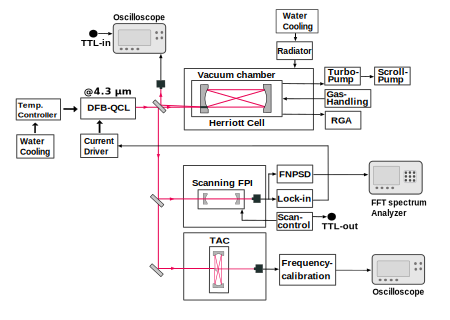
\includegraphics[width=1\textwidth]{/Absorptionspectroscopy_setup_drawing/Schematic_absorptionspectrosopy_setup_BESSER}
	\caption{Experimental setup with all optical and electrical components used for TDLAS}
	\label{fig:experimental_setup_sketch}
\end{figure}
\noindent
A \textbf{DFB-QCL} (Alpes Model:) is used as a light source in the mid infrared region (4.3$\mu$m / 2160cm$^{-1}$). Electrical noise has a significant influence on the laser linewidths, which in turn is relevant for the determination of the integrated absorbance. It is therefore crucial to minimize all electrical noise when applying voltage or current ramps to the laser in order to scan over it's frequency. Therefore a \textbf{low noise current driver} (ppq-Sense: Model QubeCl 500) is used to drive the QCL and optimize its performance. The QCL has an internal Peltier element which can be used to modulate the laser temperature between -20$^{\circ}$ and 25$^{\circ}$ Celsius. The thermometric cooler is mounted onto a water-coooled heat sink which dissipates the generated heat away from the QCL. \\\\
\noindent
To further reduce the Laser linewidths, the QCL emission is phase-locked to a \textbf{Fabry-Pérot cavity} mode (Thorlabs: Model: 	
SA200-30C). The laser-locking is achieved digitally, with a Field-Programmable-Gate-Array chip (FPGA) (Toptica: Model: Digilock), that allows the implementation of the \textbf{Lock-In} and Pound-Drever-Hall techniques. The FPGA voltage output is connected to the current modulation input of Laser driver and creates a feedback loop between the signal that is transmitted through the FPI cavity and the emission frequency of the QCL. (The Laser frequency can be adjusted by increasing or decreasing the current that is applied to the Laser). The pid controller of the FPGA modulates the output frequency of the QCL until it  perfectly overlaps with the transmission frequency of the TEM$_{00}$-mode of the FPI. By constantly forcing the QCL emission frequency onto the narrow FPI-maximum transmission frequency, one can very effectively reduce the Laser linewidths even further.\\\\
\noindent
The disadvantage of locking a laser to stable frequency reference is, that it can not be tuned directly anymore. This is due to the pid controller of the FPGA that constantly counteracts any external frequency modulation, including those that are applied directly to the Laser driver modulation input by current or voltage ramps. For TDLAS however the tuning of the laser frequency over the absorption line is required and one has to achieve it by indirectly tuning the Laser frequency. This is done by modulating the lengths of the FPI cavity to which the QCL is locked to. The \textbf{scanning-FPI} includes a piezoelectric transducer which can be compressed and expanded to reduce or increase the FPI lengths. By changing the lengths of the FPI, the Free Spectral Range (FSR) of the FPI changes ($\Delta\lambda_{FSR}=\frac{\lambda^2}{n\cdot L}$) and therefore the frequency position of the TEM$_{00}$ mode to which the laser is locked changes as well.  This procedure allows for a smooth indirect tuning of phase-locked QCL. The voltage ramp, that is applied to the FPI piezoelectric transducer can then be used as a trigger input for the absorption measurement.\\\\
\noindent
The Laser light exiting the QCL is split, using beam splitters. A small portion of the light is used to stabilize the Laser-frequency using the Lock-In technique and measure the relative frequency change. Most of the light however is coupled into the \textbf{Herriott-Cell}, where the absorbing gas is present and the measurements are performed. Depending on the configuration of the Herriott Cell and the respective distance of the Herriott-Cell mirrors to each other, optical path length between 2 and 100m can be achieved. The Herriott Cell is integrated into a 40 liter stainless steel \textbf{vacuum chamber}, that is evacuated with a turbomolecular pump and a membrane pump. The Light that exits the Herriott Cell is focused onto a detector (Thorlabs: Model PDA07P2) and filtered using a \textbf{Lock-In amplifier} (Stanford Research Systems: Model: SR850). \\\\
\noindent
Since the absorption signal A$_{line}$ is integrated over the frequency that the laser scanned, it is necessary to have precise information of the relative frequency change during the QCL-scan. Therefore a second transversally coupled Herriott-Cell (\textbf{TAC}) is used as an interferometer. The optical path length of the TAC is well known. And by measuring the interference fringe distances one can very precisely determine the relative frequency change. \\\\
\noindent
The \textbf{measurement gas} (CO with a purity of 3.7 or 4.7) is injected into the measurement chamber through a needle valve which allows the setting of very small partial pressures. After connecting the gas bottle to the system the connecting tubes were purged with CO more than five times to eliminate potential gas impurities. The exhaust of the membrane pump was directly connected to the ventilation port of the laboratory to avoid accumulation of CO in the optical pathway (outside of the Herriot Cell) and inside the laboratory. A \textbf{mass spectrometer/RGA} (MKS: Model: Vision-2000) is connected to the vacuum chamber to measure the overall Measurement gas composition and to detect vacuum leaks or gas impurities.\\\\
\noindent
Three different \textbf{pressure sensors} are used to assess the pressure when linestrength measurements are performed. A spinning rotor gauge (SRG) (Ph-instuments: Model: VIM-2) is used for the low pressure range between  10$^{-5}$ and 10$^2$ Pa. A capacitive diaphragm gauge (CDG) (MKS: Model:	AA06A, 1 Torr )  covers 10$^{-1}$ to 10$^2$ Pa and the quartz based pressure standard (Parosientific: Model: Model 745) is operational between 1 and 10$^5$ Pa.\\\\
\noindent
The Vacuum chamber, as well as all optical component are placed within a \textbf{themostatized environment}. The volume is thermally insulated with the help of styrofoam plates and the temperature within the volume is controlled and stabilized with a water cooled bath (PolyScience: Mode: AP15R) and several radiators. Temperature measurements are performed with two calibrated 25 ohm Standard Platinum Resistance Thermometers (\textbf{SPRTS}) (Fluke: Model:5686-B) and a measurement bridge (Isotech: Model: MircoK 70) together with four additional \textbf{PT-100} sensors (Ludwig Schneider: Model: Physics 1000). All sensors are positioned around the vaccum chamber and are in direct contact with the stainless steel, to ensure the best thermal contact and precise gas temperature measurements.\\\\
\noindent

\section{Laser characterization}
As a preparatory measurement, the performance of the Quantum cascade Laser was investigated to ensure a stable and mode-hop free operation within the desired frequency regions. For this purpose, the laser current was increased at a constant laser temperature until an emission could be measured with a power meter (Thorlabs: Model:PM400K5). The power meter was positioned 1 cm in front of the QCL and a current of 250 mA was not exceeded for safety reasons. Figure \ref{fig:co-qcl-outputpower} shows the optical power of the laser in comparison to the applied current and the compliance voltage. The maximum optical power at a constant laser temperature of -20$^\circ$C and a current of 250 mA is around 100 mW. One can also observe that the QCL can be tuned mode hop-free within the tested parameters since no characteristic power drop with increasing current can be observed. Due to their high compliance voltage of 9-15V Quantum Cascade Laser usually require specific Laser drivers, since the widely available Laser-diode-drivers often only support a compliance voltage of 5V.
\begin{figure}[H]
	\centering
	\includegraphics[width=0.75\textwidth]{/Measurements/Laser-characterization/CO-QCL/2020-08-18-CO-QCL-Outputpower-vs-current}
	\caption{QCL output power in comparison to the applied current and compliance voltage for different Laser temperatures between -20 and +20$^{\circ}$C.}
	\label{fig:co-qcl-outputpower}
\end{figure}

\subsection{Laser tuning range}
Two additional important properties of Quantum Cascade Lasers are: their absolute emission frequency and their maximum tuning range. Both of these properties were investigated thoroughly with the experimental setup described in \ref{fig:experimental_setup_sketch}. The tuning range of the Laser is limited by the Laser driver, which has a wide-modulation input channel that translates a voltage ramp of 1V into a current ramp of 0.1 mA. Another modulation input has a finer translation of 0.01mA/V which is suitable for Laser locking. The maximum voltage that can be applied to the Laser driver is 2V.\\\\
\noindent
To investigate what a Voltage ramp of 2V translates to in terms of Laser frequency modulation, one can use a FPI as a frequency reference and monitor the transmission signal of the cavity. Figure \ref{fig:FPI_2V_scan} shows the transmission of the FPI, when a triangle function with a 2V amplitude is applied to the modulation input of the Laser Driver. Up to seven individual TEM$_{00}$ modes are visible, if the Laser is properly aligned and mode matched with the resonator. At a cavity lengths of \mbox{10 cm} the free spectral range is equal to 1.5 GHz, which results in a total current-tuning range above 10.5 GHz.
\begin{figure}[H]
	\centering
	\includegraphics[width=1\textwidth]{/Measurements/CO_spectrum_measured_and_simulated/FPI_transmission_and_scan}
	\caption{Shown is the FPI transmission, measured with a photo detector, when a periodic triangle ramp with an amplitude of 2V is applied to the modulation input of the Laser driver.}
	\label{fig:FPI_2V_scan}
\end{figure}
\noindent
A slower method of tuning the absolute laser frequency is adjusting the Laser temperature. The semiconductor chips of QCL's are often times mounted onto a Peltier element which can be both, heated or cooled depending on the direct current that is applied. Once the desired temperature is reached a pid controller stabilizes the current applied to the Peltier element and Laser temperature remains constant. Changes in the Laser temperature usually result in much larger changes of the absolute emission frequency of the QCL and can be used to tune the Laser to different absorption lines which can not be covered by a single Laser-current scan.\\\\
\noindent
Figure \ref{fig:FPI_signal_for_CO_spectrum} shows the transmission signal of the FPI while the temperature was decreased in -1$^{\circ}$C steps from +23 $^{\circ}$C to -20$^{\circ}$C. The QCL was operating at a constant Laser current of 240mA, while a saw-tooth function, with an amplitude of 2V, was constantly applied to the modulation input of the Laser driver. By changing the QCL-temperature by 1$^{\circ}$C one can tune the Laser frequency by around 4.5GHz. Which means that the last TEM$_{00}$ mode observed in the first scan configuration with I=240mA and T=23$^{\circ}$ has the same frequency as the first TEM$_{00}$ mode of the second scan with the configuration: I=240mA and T=22$^{\circ}$. \\\\
\noindent
The consecutive scan configurations in Figure \ref{fig:FPI_signal_for_CO_spectrum} are indicated by different color schemes and labeled from n=1 to 43, where n represents the change in temperature in degrees Celsius since the initial scan with T$_0$=23$^{\circ}$C. One can also observe a change in signal amplitude which is transmitted through the FPI. The signal amplitude on the detector directly scales with the Laser output power at different operating temperatures. For temperatures higher than 23$^{\circ}$C lasing of the QCL is unstable and temperatures lower than -20 $^{\circ}$C were avoided for safety reasons.\\\\
\noindent
The emission frequency of the QCL (at a fixed operating current of 240mA) can be tuned by total of 8.8 cm$^{-1}$ or 0.263 THz by changing the operating temperature. 
\begin{figure}[H]
	\centering
	\includegraphics[width=1\textwidth]{/Measurements/CO_spectrum_measured_and_simulated/FPI_signal_for_CO_spectrum}
	\caption{Shown is the FPI transmission signal for 43 consecutive Laser scans with a modulation amplitude of 2V. After each individual scan the Laser temperature was decreased by 1$^{\circ}$C, with an initial and final operating temperature of 23$^{\circ}$C and -20$^{\circ}$C respectively. }
	\label{fig:FPI_signal_for_CO_spectrum}
\end{figure}
\subsection{Absolute emission frequency}
After determining the relative frequency tuning range of the QCL, one has to determine the absolute emission frequency to identify the line position of the individual absorption line. \\\\
\noindent
For many diode Lasers with emission wavelength below 2$\mu$m this can be achieved with direct comparisons to known frequencies (e.g Helium-Neon Lasers at 633nm) or interferometric approaches like wavemeters. Since quantum cascade lasers have only been commercially available for a few years, the supply of high-quality optical components, like dielectric mirrors with high reflectivities (R$>$99.99$\%$) which are required for many interferometric setups, is limited or disproportionately expensive due to high development costs. One can however compare the experimental absorption measurements with existing, often theoretically determined, database entries like HITRAN and obtain the absolute frequency of all absorption lines in the Laser tuning range. \\\\
\noindent
To perform such a measurement, the vacuum chamber containing the Herriott-Cell was filled with a constant Carbon monoxide pressure of 18.2 Pa. This partial pressure was chosen so that absorption lines with different linestrength can be observed simultaneously. The optical pathlengths of the Herriott-Cell was adjusted to 101m and the transmission signals were measured with a photodetector. The absorbance is obtained by:
\begin{equation}
	A=-Ln(\frac{I}{I_0})
\end{equation}
where I is the frequency dependent transmission signal at a partial CO-pressure of 18.2 Pa and I$_0$ the transmission signal for a fully evacuated vacuum chamber. To compare as many experimentally obtained absorption lines with the data base as possible, it is best to scan the Laser over the complete tuning range while measuring the absorbance. The upper image of Figure \ref{fig:CO_spectrum_measured_and_simulated} illustrates a complete temperature scan of the QCL from 23$^{\circ}$C to -20$^{\circ}$C with the measured absorbances. As shown in the previous section, the chosen temperature scan corresponds to a relative frequency modulation of 8.8 cm$^{-1}$. \\\\
\noindent
The lower image of Figure \ref{fig:CO_spectrum_measured_and_simulated} shows a simulated absorbance spectrum for $^{12}$C$^{16}$O and the first three isotopologues: $^{13}$C$^{16}$O, $^{12}$C$^{18}$O, $^{12}$C$^{17}$O  at a pressure of 18.2 Pa, a gas temperature of 296 K and an optical pathlengths of 101 m. The Hartmann-Tran lineshape profile was chosen for all absorption lines, which is an expansion of the speed dependent Voigt profile and currently has the smallest residuals when compared to the respective experimental data \cite{Hartmann-Tran}. The additional absorption line parameters required for the simulation, such as self broadening coefficients, line positions or line strengths, can be accessed from the HITRAN database directly via an API (Application program interface) \cite{HitranAPI}. The frequency resolution was set to 10$^{-5}$ cm$^{-1}$ and the spectrum was simulated for absolute frequencies between 2158.2 and 2166.99 cm$^{-1}$.\\\\
\noindent
\begin{figure}[H]
	\centering
	\includegraphics[width=1\textwidth]{/Measurements/CO_spectrum_measured_and_simulated/CO_spectrum_measured_and_hitran_simulation_mit_iso_version_2}
	\caption{Shown on the top: Experimentally obtained Carbon monoxide spectrum after tuning the QCL over 8.8 cm$^{-1}$ via its operating temperature. An optical pathlength of 101 m and a pressure 18.2 Pa were created inside the vacuum chamber.\\ Shown on the bottom: Simulated CO spectrum for an optical path lengths of 101 m and a pressure of 18.2 Pa, based on the corresponding CO-lineshape parameters of the HITRAN data base. The CO isotope responsible for the respective radiative transition is indicated and color coded.}
	\label{fig:CO_spectrum_measured_and_simulated}
\end{figure}
\noindent
Comparing the experimentally obtained absorption spectrum from the upper image, with the simulated Carbon monoxide spectrum from the Hitran data base on the lower image in Figure \ref{fig:CO_spectrum_measured_and_simulated}, one can see that the observed absorption line positions are nearly identical. A small deviation of the absorption signals can be observed at 2158.2 cm, where the Laser has has very little optical output power and therefore the signal to noise ratio is unfavorable. \\\\
\noindent
The relative position of the experimental absorption line position can now be assigned to the theoretical position from the database, by plotting the respective experimental and theoretical line positions against each other, as is shown in Figure \ref{fig:CO_spectrum_linear_Fit_with_Hitran_data}.
\begin{figure}[H]
	\centering
	\includegraphics[width=0.75\textwidth]{/Measurements/CO_spectrum_measured_and_simulated/CO_spectrum_linear_Fit_with_Hitran_data}
	\caption{Shown is the relationship between the measured peak position of the CO absorption lines in the scanning range of the QCL with the theoretically simulated peak positions obtained from the HITRAN data base.}
	\label{fig:CO_spectrum_linear_Fit_with_Hitran_data}
\end{figure}
\noindent
The linear relation indicates that the experimentally observed absorption line sequence matches with the one obtained from the HITRAN database. This observation allows for an absolute frequency assignment to all observed experimental CO-absorption lines, since a random match to another absorption line sequence can be excluded.
\section{Determination of the required Laser linewidth}
To perform accurate measurements of the line strength S or the partial gas pressure p with the absorption law (using TDLAS):
\begin{equation}
	A_{\text{line}} = S\cdot n \cdot L = S \cdot \frac{p}{k_B\cdot T} \cdot L
\end{equation}
it is necessary to evaluate the uncertainty contribution of the integrated absorption A$_{{\text{line}}}$, optical path-length L and the gas temperature T. While the temperature and path-length uncertainties can be accessed directly by their respective measurement device calibration, the uncertainty of the integrated absorbance has to be determined based on the measurement Laser properties. Namely the Laser-linewidth. During the measurement (using a TDLAS setup) the laser is tuned over an isolated absorption line. Since the laser has a finite linewidth the measured integrated absorbance will always deviate from the theoretically expected one. \\ \\ The discrepancy between the theoretical expectation and experimental result can be simulated by comparing the two with each other. To define a theoretical value for the comparison, a CO$_2$ absorption line at 4.305 $\mu$m was taken from the HITRAN database. The absorbance and transmittance for said absorption line were determined based on the properties given in the database. The absorption-line broadening was calculated for room temperature (296K) and a pressure of $1 \cdot 10^{-5}$ mbar. The linewidth of the assumed Voigt profile is in the order of $3.8 \cdot 10^{-6} \mu$m. The theoretically expected absorbance A$_{{\text{line}}}$ was then calculated by integrating over the absorption line.\\ \\ The expected experimental result was generated by simulating the measurement process directly. Therefore a Gaussian Laser profile was swept over the HITRAN-CO$_2$-absorption line. The convolution integral of the sweeping Laser (L$_{\text{aser}}$) and the transmission curve of the absorption line (T$_{\text{Hitran}}$) yields the expected experimental result for the transmittance ($\text{T}_{\text{Exp}}$).

\begin{equation}
	\text{T}_{\text{Exp}}(\lambda) =(\text{L}_{\text{aser}} * \text{T}_{\text{Hitran}})(\lambda) = \int_{-\infty}^{\infty} T(\tau) \cdot L(\lambda -\tau)  d\tau
\end{equation}
The expected experimental result for the absorbance ($\text{A}_{\text{Exp}}$) can then be calculated from the determined transmitance.
\begin{equation}
	\text{A}_{\text{Exp}}  = \frac{-\text{log}(\text{T}_{\text{Exp}})}{\text{L} \cdot \text{c}} 
\end{equation}
The influence of the Laser on the measurement accuracy was then determined by performing the simulation with varying Laser linewidth. The starting Laser-HWHM of: $3.8 \cdot 10^{-6} \mu$m was gradually reduced to its the final value of  $3.8 \cdot 10^{-9} \mu$m. The expected experimental and theoretical values of the absorbance and transmittance can then be compared and used to determine the uncertainty contribution ($\delta \text{A}$ and $\delta \text{T}$) of the Laser. 
\begin{align}
	\begin{split}
		\delta \text{A} &= \left| \int_{-\infty}^{\infty} \text{A}_{\text{Exp}} \text{ d}\lambda - \int_{-\infty}^{\infty}\text{A}_{\text{Theo}} \text{ d}\lambda \right| \\
		\delta \text{T} &= \left|\int_{-\infty}^{\infty} \text{T}_{\text{Exp}} \text{ d}\lambda - \int_{-\infty}^{\infty}\text{T}_{\text{Theo}} \text{ d}\lambda  \right| \\
	\end{split}
\end{align}
The results of the simulation are summarized in Fig. \ref{C02_pressuredependant_linewidth_1} and Table \ref{Laser_HWHM_table}.
\begin{figure}[H]
	\centering
	\includegraphics[width=0.95\textwidth]{/HITRAN-Linewidth-and-absorption/Simulated_absorption_and_transmission}
	\caption{Shown are the experimentally expected (red) and the theoretically expected (blue) transmission and absorption curves of a CO$_2$ line, which is centered around 4.305 $\mu$m. From top to bottom the corresponding Laser-linewidth are $3.8 \cdot 10^{-6}$, $3.8 \cdot 10^{-7}$ and $3.8 \cdot 10^{-9}$. The individual uncertainty contributions ($\delta$T and $\delta$A) are displayed together with the Laser-linewidth that was used for the respective simulation iteration. }
	\label{C02_pressuredependant_linewidth_1}
\end{figure}
\begin{table}
	\begin{center}
		\begin{tabular}{ lllll }
			\toprule
			Laser HWHM ($\mu$m): & $3.8 \cdot 10^{-6}$ & $3.8 \cdot 10^{-7}$ & $3.8 \cdot 10^{-8}$  & $3.8 \cdot 10^{-9}$ \\
			\midrule
			$\delta$T (arb. units): & $9.0 \cdot 10^{-2}$& $3.0 \cdot 10^{-5}$& $1.4 \cdot 10^{-6}$ &  $1.2 \cdot 10^{-7}$\\
			$\delta$A (arb. units): &$1.2 \cdot 10^{0}$&$9.7 \cdot 10^{-3}$&$1.6 \cdot 10^{-4}$&$5.9 \cdot 10^{-5}$\\
			\bottomrule
		\end{tabular}
	\end{center}
	\caption{Comparison of different Laser-linewidths and their influence on the uncertainty contributions $\delta$T and $\delta$A. The target uncertainty of $10^{-4}$ for $\delta$A is reached with a Laser-linewidth of $3.8 \cdot 10^{-9}\mu$m.}
	\label{Laser_HWHM_table}
\end{table}
\noindent
By reducing the linewidth of the Laser one can  continuously decrease the uncertainty contribution $\delta$A to the integrated absorbance A$_{\text{line}}$. The target uncertainties for partial pressure and linestrength measurements within the QuantumPascal project are in the order of $10^{-4}$, when carried out with a TDLAS setup. To achieve these goals the linewidth of the quantum cascade Laser has to be at least three orders of magnitude smaller than the linewidth of the measured absorption line. Since the absorption line broadening depends on pressure, emission frequency and temperature, the exact Laser-linewidth that is required has to be calculated for each case individually. For simplicity purposes it would also be acceptable to assume a Gaussian profile for the absorption line at 4.305 $\mu$m. Assuming that the pressure in the measurement chamber is below 1 Pa. Figure \ref{C02_pressuredependant_linewidth} compares the contribution of the Gaussian and Lorentzian line-broadening to the total absorption-line linewidth. Up to a pressure of 1 Pa the pressure dependent Lorentzian line broadening is at least three orders of magnitude smaller than the temperature dependent Gaussian line broadening.
\begin{figure}[H]
	\centering
	\includegraphics[width=0.75\textwidth]{/HITRAN-Linewidth-and-absorption/Druck-Linienbreite(296K)_v=4_305_fullscale}
	\caption{The graphic illustrates the pressure dependent absorption linewidth broadening for an exemplaric CO$_2$ line at 4.305 $\mu$m. Shown are the Gaussian, Lorentzian and the total linewidth from the high vacuum region up to atmospheric pressure. All data was taken from the HITRAN database \cite{Hitran2012} \cite{Hitran2016}.}
	\label{C02_pressuredependant_linewidth}
\end{figure}
\newpage
\section{Reducing Laser-linewidths and Laser locking}
As shown in the previous sections, Quantum cascade Laser provide an excellent single mode tuning range at high optical output powers. The intrinsic linewidth for quantum cascade lasers is given by the Schawlow-Townes limit \cite{Shawlow-Twones} and is caused by white noise. It can be as low as a few Hertz and depends on several factors:
\begin{equation}
	\Delta \nu_{QCL}=\frac{4\pi h \nu (\Delta \nu_c)^2}{P_{out}}
\end{equation}\\
The photon energy $h\nu$, the output power of the Laser $P_{out}$ and the laser-resonator bandwidth $\Delta \nu_c$. Additional noise from other sources, like thermal or electrical noise from the Laser driver, further broaden the emission linewidth of semiconductor Lasers. If these noise sources are not addressed, the typical emission linewidth of a QCL is in the order of a few Mega Hertz, which is several orders of magnitude higher than the theoretical lower limit predicted by Schawlow and Townes. Since narrow linewidth Laser sources in the MIR are crucial for high resolution spectroscopic applications, extensive research has been performed in the last several years. Mainly with the goal to: quantify the influence of frequency noise on the Laser Linewidth \cite{DiDomenico-2010} and reduce Laser linewidth with different experimental approaches. Such as locking a Laser to: an optical delay line \cite{Shezad-2019}, micro resonators like a whispering Gallery \cite{deCumis-2016}, V-shaped cavities \cite{Fasci-2014}, MIR frequency combs  or sub-doppler CO$_2$ transitions \cite{Cappelli-2012}. \\\\
\noindent
The Laser linewidth optimization approach, chosen for this thesis, combines an ultra low current noise Laser driver with locking the QCL to a high finesse Fabry Pérot cavity. The low noise Laser driver is required to minimize electrical noise that is applied to the semiconductor chip when tuning or running the QCL. The optical lock to a FP-cavity is implemented to further reduce the frequency noise by stabilizing the Laser to an optical frequency reference, namely the sharp transmission peaks (TEM$_{00}$ modes) of the resonator. \\\\
\noindent
Figure \ref{fig:QCL_FPI_tranmission} shows the transmission signal of a single TEM$_{00}$ mode of the FP-cavity which is used for locking the QCL. Since the TEM$_{00}$-mode transmissions are separated in frequency by 1.5 GHz (cavity length of 10 cm), one can tune the absolute emission frequency of the laser to any arbitrary value, by changing the operating temperature, and then lock it to the closest TEM$_{00}$- mode of the FP-cavity. \\\\

\begin{figure}[H]
	\centering
	\includegraphics[width=0.99\textwidth]{/Measurements/FPI_QCL_Scan_and_lock/FPI_transmission_and_LOCK}
	\caption{Shown are the transmission signals behind the FP-Cavity, before the lock is engaged (blue), after the lock is closed (black) and the generated error-signal (red).}
	\label{fig:QCL_FPI_tranmission}
\end{figure}
\noindent
To stabilize the Laser frequency to the FP-cavity reference, the Lock-In technique was used which could be implemented digitally by using a FPGA-chip (Toptica: Digilock) which itself is connected to the Laser driver. The FPGA has two modulation output channels, which allow scanning of the Laser frequency by applying voltage ramps to the modulation input of the Laser driver. On the first output channel of the FPGA a periodic triangle function with an amplitude of 0.2 V is applied. The scanning amplitude is chosen so that only one transmission peak can be observed on the detector as is shown in Figure\ref{fig:QCL_FPI_tranmission}. \\\\
\noindent
For the Lock-In technique to work, a second, fast modulation channel is required. Figure \ref{fig:LOCK-in_experimental_setup} illustrates the operating principle of the Lock-In technique. The FPGA applies a fast (between 1kHz and 1 Mhz) demodulation with a very small amplitude to the second input channel of the Laser driver. By quickly demodulating the signal, one can generate the derivative of the input signal that is observed on the detector. This, experimentally obtained, derivative signal can then be used as an Error signal for a pid controller. The pid controller takes the Error signal as information input and optimizes the voltage, applied to the fast input channel of the Laser driver. So that the emission frequency of the Laser is constantly forced to the center frequency of the TEM$_{00}$ mode. This  works since the error function has a zero crossing at the peak position of the Cavity transmission signal and the pid controller is set to stabilize the error signal to zero. Once the Lock is engaged, the slow modulation on the first channel can be turned off and instead be used to compensate for slow frequency changes (e.g cause by temperature changes)\\\\

\begin{figure}[H]
	\centering
	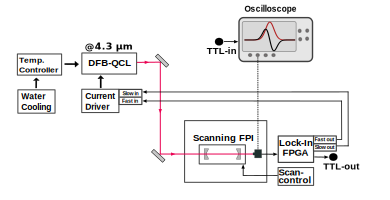
\includegraphics[width=0.75\textwidth]{/Absorptionspectroscopy_setup_drawing/Schematic_LOCK_IN_setup_BESSER}
	\caption{Shown is the basic operating principle of the Lock-In technique as it was implemented in this thesis, together with all optical and electrical components that were required.}
	\label{fig:LOCK-in_experimental_setup}
\end{figure}
\noindent
The disadvantage of locking a Laser to an external frequency reference is that it can not be directly tuned in its emission frequency anymore. Since this property is important for TDLAS, one can instead tune the frequency reference to which the Laser is locked to. This allows for an indirect frequency modulation of the Laser while still benefiting from the linewidth narrowing of the Laser Lock. When using a Fabry Pérot cavity as a frequency reference this indirect tuning can be achieved by changing the length of the resonator. FP-cavities are often times used as a scanning Fabry Pérot interferometers and come with an integrated piezoelectric transducer. This transducer is used to periodically modulate the cavity length by compressing an expanding the transducer with the help of periodic voltage ramps. When the QCL is locked to a TEM$_{00}$- mode of the FP-cavity and the cavity length is periodically modulated, the indirect modulation of the emission frequency is achieved. However, these piezoelectric transducers often times tune the Laser frequency in a non-linear fashion due to hysteresis effects during the scan. Therefore additional care is required when calibrating the emission frequency of the Laser.
\section{Frequency calibration}
\label{sec:frequency_calibration}
For TDLAS, the measured absorption signals are generally integrated over the frequency, to obtain the integrated absorption: A$_{line}$ of the signal. This requires precise knowledge of the relative frequency change while the Laser is scanned. To achieve this, a transversally coupled Herriott-Cell (TAC) was used as an optical interferometer and absolute frequency standard. The laser light enters the TAC perpendicular to the classical optical axis, as is shown in Figure \ref{fig:TAC_experimental_setup} which illustrates the parts of the experimental setup that are required to calibrate the frequency axis. The laser light is coupled in and out of the TAC with the help of a very thin and highly reflective silver-plate. The silver plate is positioned, so that only 50 percent of the Laser light is coupled into the Herriott cell with an optical pathlength of 6.429589 m and the other 50 percent are sent directly onto the photodetector. During a measurement the QCL is tuned i its emission frequency and one can observe an interference pattern on the detector where the interference fringes are separated in frequency by:
\begin{equation}
	\Delta \nu_{TAC}= \frac{c}{n\cdot L}
\end{equation}\\
where n is the refractive index of the gas, L is the optical pathlength of the TAC and c is the speed of light. To avoid density fluctuations and decrease vibrations, which negatively influence the interference signal, the TAC is integrated into a UH-vacuum chamber and placed on a vibration damped optical table.
Assuming that the refractive index in vacuum is 1, one obtains a frequency separation of the individual interference fringes of $\Delta \nu_{TAC}$ =46.627 MHz.
\begin{figure}[H]
	\centering
	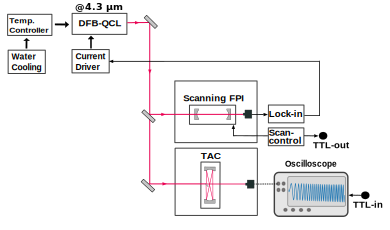
\includegraphics[width=1\textwidth]{/Absorptionspectroscopy_setup_drawing/Schematic_TAC_fringe_measurement_BESSER}
	\caption{}
	\label{fig:TAC_experimental_setup}
\end{figure}
\noindent
As shown in the previous section, the QCL is locked to a Fabry-Pérot resonator to narrow the Laser linewidth by reducing the frequency noise. In order to tune the Laser while it is locked, the Fabry-Pérot length is periodically modulated. This experimental approach results in a slightly nonlinear tuning of the Lasers emission frequency, which has to be considered when calibrating the frequency axis. (And should be considered even for direct tuning of the Laser since self heating effects can cause non-linear tuning as well). Figure \ref{fig:TAC_interference_pattern} shows the interference signal that is obtained on the photo detector behind the TAC. The length of the FPI was modulated at a high frequency of 200 Hz and the shown signal covers the first 1.7 ms of the scan, where the non-linearity is most significant. \\\\
One can then perform a fast Fourier transformation of the interference pattern to visualize the frequency change during the QCL-scan.  The result of the FFT is visualized in a spectrogram which plots the current frequency of the time series against the respective measurement time. The spectrogram reveals a clearly visible non-linear chirp of the time series. This chirp was then interpolated, rather than fitted as the functional relationship is not fully known due to many simultaneously occurring effects (e.g self heating or hysteresis effects of the piezo). With the interpolated chirp signal one can then correct and linearize the interference signal together with the measured absorption signals. The linearized signal is shown in Figure \ref{fig:TAC_interference_pattern} on the right.\\\\
\begin{figure}[H]
	\centering
	\includegraphics[width=1\textwidth]{/Measurements/TAC_frequency_axis_correction/TAC_signal_corrected_uncoreccted}
	\caption{Shown on the top left: The measured interference signal for the first 1.7 ms of the scan duration.\\
	Shown on the bottom left: Shown is the spectrogram of the interference signal.\\
	Shown on the top right: Linearized signal after correcting for the chirp.\\
	Shown on the bottom right: Spectrogram of the corrected interference signal.}
	\label{fig:TAC_interference_pattern}
\end{figure}
\noindent
An alternative method to the Fourier analysis is a direct investigation of the interference pattern. One can obtain the inverse of the correction function by plotting the interference peak distance against the respective measurement time.
\newpage
\section{Temperature assessment}
The vacuum chamber containing the measurement gas is integrated into a fully themostatized environment, which is shielded against room temperature fluctuations with a Styrodur enclosure. A precision water bath can be used in combination with several radiators to stabilize the temperature inside the enclosure (and inside the vacuum chamber) to any arbitrary temperature close to room temperature (between 21-24 $^{\circ}$C). Figure \ref{fig:roomtemperature_stabilization} shows the temperature inside the the enclosure with and without active cooling for a several hour-long time period.
\begin{figure}[H]
	\begin{subfigure}[t]{.48\textwidth}
		\centering 
		\includegraphics[width=\linewidth]{/Measurements/Thermostatisation_temperature_stability/Temperature_stability_thermostatisation_without_active_cooling}
		\caption{No active cooling: Shown is a comparison of the room temperature in the laboratory and the temperature within the thermal insulation for the time period from 24.2.2021 to 03.03.2021. The room temperature follows the outdoor temperature since the AC is not properly adjusted. The thermal insulation results in a delayed temperature increase/decrease with significantly less total amplitude change.\hfill}
		\label{fig:roomtemp_1}
	\end{subfigure}
	\hfill
	\begin{subfigure}[t]{.48\textwidth}
		\centering
		\includegraphics[width=\linewidth]{/Measurements/Thermostatisation_temperature_stability/Temperature_stability_thermostatisation_with_active_cooling}
		\caption{With active cooling: The PID control of the AC was adjusted and an active temperature control was added within the thermal insulation.}
		\label{fig:roomtemp_2}
	\end{subfigure}
\caption{Temperature profiles within the thermally insulated enclosure.}
\label{fig:roomtemperature_stabilization}
\end{figure}
\noindent
The temperature stability within the thermal insulation was better than 25 mK (peak to peak) for a 38 hour long period. \\\\
\noindent
During TDLAS measurements, the gas temperature is assessed with two 25 Ohm standard platinum resistance thermometers (SPRT) which are connected to a measurement bridge (Isotech:MircoK 70) and a reference resistor. Over a period of 2 years, the SPRTs were calibrated three times against the water triple point and the Gallium melting point in the temperature laboratory of the PTB. During the calibration, the same measurement bridge was used, which compensates for the self heating of the SPRT-sensors which require an operating current of 1 mA. The resistance of the SPRT is assessed with a four wire measurement and then internally compared to the reference resistor. The reference resistor itself is integrated into a temperature controlled box which operates at 23 $^{\circ}$C. With the help of the calibration certificate the measured resistances of the SPRTs can then be converted into temperatures.\\\\
\noindent
The SPRTs together with four additional PT100 sensors are then put in direct contact with the vacuum chamber to assess the temperature profile of the gas during the TDLAS measurement. The PT100 sensors were calibrated against the SPRTs in a high precision calibration bath (CIK: Kambic) with a temperature stability of 1 mk.
\section{Pressure assessment}
\label{sec:Pressure_assessment}
During the linestrength assessment the Carbon monoxide pressure was modulated to approach and measure different pressure points. Pressure increases were adjusted using a needle valve while pressure decreases were realized with pumping out the gas with the help of a turbomolecular pump. Figure \ref{fig:pressure_modulation} shows an exemplaric pressure modulation for TDLAS measurement campaign.
\begin{figure}[H]
	\centering
	\includegraphics[width=0.75\textwidth]{/Measurements/Pressure_modulation/pressure_step_exemplaric_ABS_measurement}
	\caption{Exemplaric pressure modulation.}
	\label{fig:pressure_modulation}
\end{figure}
\noindent
The pressure is increased step wise until an arbitrarily chosen maximum value is reached and then decreased again so that similar pressure values can be assessed under different experimental conditions. This is done to ensure that the pressure modulation and demodulation has no influence on the experimentally determined absorption: A$_{line}$. After every modulation cycle a zero measurement is performed, which is later used to determine the transmission intensity I$_0$, when no gas is present within the multipass absorption cell.\\\\
\noindent
Pressure measurements are carried out with one of three different pressure sensors. The sensors cover different pressure regions and are chosen accordingly to achieve the lowest uncertainties and highest performance. A Spinning rotor gauge (SRG, 10$^{-5}$ to 10$^2$ Pa), Capacitive Diaphragm Gauge (CDG, 10$^{-1}$ to 10$^2$ Pa) and a quartz based pressure standard (1 and 10$^5$ Pa) were used. The CDG and the Quartz based standard were calibrated in the pressure department of the PTB and have been compared to the state of the art static expansion system.
\subsection{Thermal transpiration effects}
For many pressure measurements, between between 10$^{-2}$ and 100 Pa, a capacitive diaphragm gauge (CDG) was used.
CDG's are sensitive to temperature variation and are therefore often times operated and stabilized to temperatures above room temperature (generally between \mbox{40 and 45 $^{\circ}$C}). Due to the temperature difference between the vacuum chamber and the pressure sensor one can observe the so called thermal transpiration effect. If the CDG is connected to the vacuum chamber via a tube, the pressure P$_2$ of the sensor is not equal to the pressure P$_1$ inside the vacuum chamber if the overall pressure is low enough for the system to be in the molecular regime\cite{Setina-1999}.\\\\
\noindent
Wether the system is in the molecular or continuous regime is defined by the Knudsen number, which is given as the ratio of the mean free path lengths of the gas particles ($\lambda$) with respect to the connecting tube diameter (d):
\begin{equation}
	K_n= \lambda/d
\end{equation}
For Knudsen numbers grater than 10, the system is in the molecular regime. Between 0.1 and 10 one can observe the transitonal flow and for Knudsen numbers below 0.01 the system is in the continuous regime.\\\\
\noindent
If the mean free path of the gas molecules is much grater than the tube diameter (molecular regime) the ratio of the two pressures P$_1$ and P$_2$ are equal to the Knudsen number:
\begin{equation}
	K_n= \frac{P_2}{P_1}= \sqrt{\frac{T_2}{T_1}}
\end{equation}
while they are equal in the continuous regime. For the intermediate region, between the molecular and the continuous region the thermal transpiration value $\frac{P_2}{P_1}$ ranges between the two extremes \cite{Takaishi-1963}. \\\\
\noindent
For precise pressure measurements with CDGS below 10 Pa, knowledge of the thermal transpiration ratio is crucial. Knowledge of this effect can be obtained by calibrating the CDG against a pressure standard like the continuous-expansion-system, which does not operate at elevated temperatures. Figure \ref{fig:CDG_calibration} shows the respective calibration data which illustrates the thermal transpiration effect as well. The deviation between the two pressure values P$_1$ and P$_2$ can be as large as 4 \%. Using the calibration data as a correction of the measured CDG-pressure allows the thermal transpiration effect to be excluded and corrected in all further measurements. The calibration was performed by the Vacuum Metrology working group of the PTB.
\begin{figure}[H]
	\centering
	\includegraphics[width=0.85\textwidth]{/Measurements/CDG-calibration/CDG_calibration}
	\caption{Shown is the calibration data of the CDG used for pressure measurements during this thesis. The pressure ratio P$_2$/P$_1$ is plotted over the respective calibration pressure to illustrate the thermal transpiration effect over a wide pressure range.}
	\label{fig:CDG_calibration}
\end{figure}
\section{TDLAS measurements}
After the preliminary experiments were conducted and the experimental system was characterized, TDLAS measurements were performed to investigate the linestrength $S$ of Carbon Monoxide in the spectral region from 2158 and 2170 cm$^{-1}$, with the complete experimental setup shown in \ref{fig:experimental_setup_sketch}. The linestrength of any absorption line in the spectral region can be obtained by measuring the integrated absorbance $A_{line}$ against the respective gas pressure $p$:
\begin{equation}
	S = \frac{A_{\text{line}}  k_B T }{p L}
\end{equation}
\noindent
With knowledge of the gas temperature $T$ and the absorption pathlength $L$, one can obtain the linestrength S from the linear relationship of the measure parameters.
\subsection{Pressure dependent transmission and absorption signals}
For an initial linestrength measurement, the QCL was tuned to an emission frequency of \mbox{2165.6 cm$^{-1}$} and locked to the closest TEM$_{00}$ mode of the Fabry Pérot cavity. The FPI was then indirectly tuned so that the emission frequency of the Laser could be scanned over \mbox{0.062 cm$^{-1}$}.The non-linear frequency tuning was compensated for by the technique described in section \ref{sec:frequency_calibration}. The CO gas pressure was step wise increased from 0.2 to 5 Pa during the measurements and the respective transmission and absorption curves are shown in Figure \ref{fig:trans_and_abs_signals}. The transmission intensity $I_0$ is obtained on the detector when the vacuum chamber is completely evacuated.
\begin{figure}[H] 
	\begin{subfigure}[t]{.48\textwidth}
		\centering 
		\includegraphics[width=\linewidth]{/Measurements/CO-linestrength/Tranmissions_signals_different_pressures_1}
		\caption{Transmission signals for CO around \mbox{2165.6011 cm$^{-1}$}}
		\label{fig:transmission_signals_1}
	\end{subfigure}
	\hfill
	\begin{subfigure}[t]{.48\textwidth}
		\centering
		\includegraphics[width=\linewidth]{/Measurements/CO-linestrength/Absorption_signals_different_pressures_1}
		\caption{Absorption signals for CO around \mbox{2165.6011 cm$^{-1}$}}
		\label{fig:absorption_signals_1}
	\end{subfigure}
	\caption{}
	\label{fig:trans_and_abs_signals}
\end{figure}
\noindent
One can observe that both, the transmission and absorption signals scale with increasing pressure. However, only the absorption scales linearly with pressure due to the non-linear relation ship between the transmission and absorption. \\\\
\subsection{Comparison with simulation and fitting models}
To obtain the integrated absorbance A$_{line}$, one can either directly integrate the experimental data or fit the experimental data with an appropriate line shape function e.g a Gaussian-, Lorentz-, Voigt- or Hartmann-Tran-profile. Where the Hartmann-Tran profile \cite{Hartmann-Tran} is the currently recommended line-shape standard (e.g by the HITRAN community), as it accounts for most currently known effects that further alternate the natural line shape. \\\\
\noindent 
Figure \ref{fig:lineshape_fit_models_1_5Pa} and \ref{fig:lineshape_fit_models_6_61Pa} show the absorption signal of two individual measurements at a partial CO-pressure of \mbox{1 Pa} and \mbox{5 Pa} respectively. The experimentally obtained data is then compared a simulated absorption spectra utilizing the Hartmann-Tran profile and three different fitting models (Gaussian, Lorentz, Voigt). The simulated spectra were generated with the same environmental influences, that were present during the experiment: A gas temperature of 296K, a pressure of \mbox{1 (or 5) Pa} and an absorption pathlength of \mbox{101 m}. The remaining gas parameters, required for the simulation, could be obtained from the HITRAN database directly. 
\begin{figure}[H]
	\centering
	\includegraphics[width=0.85\textwidth]{/Measurements/CO-linestrength/Absorption_with_differetn_fit_models_1_51Pa}
	\caption{Absorption spectrum of CO at a pressure of \mbox{1 Pa} in comparison with four different models.}
	\label{fig:lineshape_fit_models_1_5Pa}
\end{figure}
\noindent
The residuals obtained from comparing the experimental data set with the respective fits and the simulation are shown at the bottom of \ref{fig:lineshape_fit_models_1_5Pa}. As expected, for pressures far below \mbox{100 Pa}, the Lorentzian broadening is small which results in the greatest residuals  for the Lorentzian fitting model. At a pressure of 1 Pa the pressure induced Lorentzian broadening makes up for less than a percent of the total spectral line broadening of the absorption signal. Which means that for small pressures a Gaussian and a speed-dependent-Voigt model yield similar results and the residuals of the Voigt model are only slightly lower than that of the Gaussian fit. For higher pressures, e.g \mbox{5 Pa}, as shown in Figure \ref{fig:lineshape_fit_models_6_61Pa} the difference in the residuals between the Gaussian and Voigt fitting approach are more significant.
\begin{figure}[H]
	\centering
	\includegraphics[width=0.85\textwidth]{/Measurements/CO-linestrength/Absorption_with_differetn_fit_models_6_61_pa}
	\caption{Absorption spectrum of CO at a pressure of \mbox{5 Pa} in comparison with four different models.}
	\label{fig:lineshape_fit_models_6_61Pa}
\end{figure}
\noindent
When looking at the residuals between the experimental data and the theoretical simulation, one can observe a similar characteristic as with the Gaussian and Voigt fit. Initially it seems as the residuals are overall deficient, however when integrating over the complete spectrum the total integrated residuals of the theoretical simulation are superior to those of obtained from the two fitting models. Table \ref{table:fitting_residuals_abs} summarizes the comparison of the experimental data with the simulation ad fitting models.
\begin{table}
	\begin{center}
		\begin{tabular}{ lllll }
			\toprule
			Fitting model / Simulation: & Lorentzian & Gaussian & SD-Voigt  & Hartmann-Tran-sim. \\
			\midrule
			Integrated residuals: & xx& xx& xx &  xx\\
			\bottomrule
		\end{tabular}
	\end{center}
	\caption{Comparison between different fitting approaches and theoretical simulation.}
	\label{table:fitting_residuals_abs}
\end{table}
\\\\
\noindent
After choosing the fitting model which yields the smallest deviation from the experimental data, one can then either integrate over the respective fitting function or directly integrate the experimental data to obtain A$_{line}$. 
\subsection{Carbon monoxide line strengths}
Experimental linestrength measurements for Carbon monoxide were carried out for five different absorption lines in the spectral region between \mbox{2158 and 2170 cm$^{-1}$}. Including three R-branch transitions of $^{12}$C$^{16}$O, one R-branch transition of the first isotopologue $^{13}$C$^{16}$O and another R-branch transition of second isotopologue $^{12}$C$^{18}$O. \\\\
\noindent 
Since the individual absorption lines, in the observed frequency region, have significantly different linestrengths (between  10$^{-23}$ and 10$^{-19}$) one has to adjust the optical path length between measurements, to investigate different absorption lines at similar partial pressure values. This is required because often times the strong absorption lines of the spectrum are already saturated before the weak absorptions can be detected. Alternatively one could operate the Herriott-Cell at the same optical pathlength for all the different absorption lines and instead utilize different calibrated pressure sensors for the respective pressure regions. However this requires extensive calibration work, for a wide array of different pressure sensors and vacuum ranges. \\\\
\noindent
During this thesis a movable, vacuum compatible Herriott cell was utilized which can be used to adjust the optical path lengths between measurements. Unfortunately the electronics required to drive the vacuum precision motor of the Herriott-Cell broke and could not be repaired in time due to consecutive global crises and the resulting supply bottlenecks. As an alternative the Herriott-Cell was tuned to an optical pathlength of 101 m and a second absorption path, with an optical pathlength of 27 cm, was created within the same vacuum chamber. These two, separate optical pathlength were chosen so that they are around four orders of magnitude apart from each other, just like the linestrength of the different absorption lines. Allowing for the observation of the strong and weak absorption line at similar partial pressures but very different optical pathlength.\\\\
\noindent
For the individual linestrengths measurements, the appropriate optical path lengths was chosen, and then the CO-pressure was adjusted to various partial pressure plateaus as described in the "Pressure assessment" section  \ref{sec:Pressure_assessment}. The integrated absorption A$_{line}$ is the plotted against the respective pressure, as well as $P\cdot L \cdot (k_b \cdot T)^{-1}$ to obtain the linestrength from the slope of the linear relation ship between the two experimentally measured properties. Figure \ref{fig:Linear_linestrength_plot_WITH_calibration} shows the measurement results for the $^{13}$C$^{16}$O absorption at \mbox{2169.198 cm$^{-1}$} together with the residuals to the linear fit. The optical pathlength for the measurement was set to \mbox{27 cm}.
\begin{figure}[H]
	\centering
	\includegraphics[width=1\textwidth]{/Measurements/CO-linestrength/Linear_linestrength_plot_WITH_calibration}
	\caption{Shown is the linestrength measurement for the $^{13}$C$^{16}$O absorption at \mbox{2169.198 cm$^{-1}$}. The second x-axis at the top  shows the respective measurement pressure. Below the linear plot, the relative measurement residuals are shown in \%.}
	\label{fig:Linear_linestrength_plot_WITH_calibration}
\end{figure}
\noindent
The experimental results for the three R-branch transitions of $^{12}$C$^{16}$O are shown in Figure \ref{fig:R-branch_transitions}. For these strong absorption lines, the Herriott-Cell with an optical pathlength of \mbox{101 m} was required and utilized.
\begin{figure}[H]
	\centering
	\includegraphics[width=1\textwidth]{/Measurements/CO-linestrength/R_branch_lines_with_hitran_inlet}
	\caption{Shown are the R-branch transitions of $^{12}$C$^{16}$O in the measurement region between \mbox{2158 and 2170 cm$^{-1}$}, together with the linear fit residuals in the lower graphic. The second x-axis at the top again clarifies the respective measurement pressure. The small inlet is shown to illustrate which absorption lines which were investigated. }
	\label{fig:R-branch_transitions}
\end{figure}
\noindent
The experimentally determined linestrengths for all measurements are compared to the Hitran values in table \ref{table:linestrengths}
\begin{table}
	\begin{center}
		\begin{tabular}{ lllllll }
			\toprule
			Line position in cm$^{-1}$: & 2161.9682  & 2165.6010 & 2169.1980 & 2164.2185 & 2162.5364 & \\
			\midrule
			Exp. linestrength: & xx& xx& xx &  xx & xx &\\
			\midrule
			Hitran linestrength: & xx& xx& xx &  xx & xx &\\
			\bottomrule
		\end{tabular}
	\end{center}
	\caption{Comparison experimental and HITRAN linestrengths.}
	\label{table:linestrengths}
\end{table}\\\\
\newpage
\section{TDLAS as a pressure standard}
With the experimentally determined linestrengths one can then use the TDLAS setup as a transfer standard for CO partial pressures. The linestrength are used as an input parameter and one can utilize the measurement formula to measure pressure: 
\begin{equation}
P = \frac{A_{\text{line}}  k_B T }{S L}
\end{equation}
Figure \ref{fig:TDLAS_pressure_range} illustrates the pressure range that can be covered with the built TDLAS system and the two different optical path lengths. Pressures as low as 7$\cdot 10^{-4}$ Pa can still be resolved at an optical pathlength of 101 m utilizing the strong absorption lines of the given spectrum. The upper pressure range is just below 100 Pa and can be covered with a weak absorption line at \mbox{2162.5364 cm$^{-1}$}. 
\begin{figure}[H]
	\centering
	\includegraphics[width=1\textwidth]{/Measurements/CO-linestrength/All_lines_vs_pressure}
	\caption{Shown is the pressure range that is covered by each individual absorption line in the given spectral region with the described optical path lengths.}
	\label{fig:TDLAS_pressure_range}
\end{figure}
\subsection{Outlook and improvements}
As shown in the previous section TDLAS can be utilized as a partial pressure standard for Carbon monoxide for a pressure range between \mbox{10$^{-4}$ and 10$^2$ Pa}. However, not the complete pressure scale can be realized with the current setup. This is due to the inability to change the optical pathlength between more than two different values (101 and 0.27 meters). With a functioning vacuum translation stage for the Herriott-Cell the optical path length can be changed much more flexible as is shown in Figure \ref{fig:Conventianal_Herriot_Cell_configurations}. The graphic was made before the translation stage was damaged and illustrates the different closed configurations of the Herriott-Cell. The distance between the two mirrors was increased by translating one mirror further away from the other and the distance change was measured with a Laser interferometer. During the translation, the Laser light intensity that was transmitted through the Herriott-Cell was observed on a photo detector. The mirrors have a finite reflectivity $R<1$ which means that the observed detector intensities directly scale with the optical pathlengths of the Herriott-Cell configurations. Many different configurations and optical pathlengths (between \mbox{1 and 101 m}) are possible, which could significantly improve the utilization of the TDLAS setup as a pressure standard. The complete pressure scale could then be covered by adjusting either the absorption line or the optical pathlengths of the Herriott-Cell or a combination of both.
\begin{figure}[H]
	\centering
	\includegraphics[width=0.9\textwidth]{/Measurements/Herriot-cell-config/2020-31-07-Ergebnis-der-Messung_1}
	\caption{Shown are the closed configurations of the Herriott-Cell for a relative change in mirror distance between 0 and 500 mm. }
	\label{fig:Conventianal_Herriot_Cell_configurations}
\end{figure}
\subsubsection{TDLAS as a total pressure standard}
The presented TDLAS was so far only used as a partial pressure standard for Carbon monoxide. It is however possible to use the same experimental setup as a total pressure standard without making any adjustments. This is possible since other gases, e.g H$_20$, have absorption lines with similar linestrengths (10$^{-23}$) as CO in the same spectral region. If a gas mixture of H$_20$ and CO is present, one can determine the partial pressure of the two gasses individually by tuning the QCL to the respective absorption line and then determine the total pressure as a sum of both partial pressure values.
\newpage
\chapter{Refractometry}
In addition to the TDLAS setup, another optical pressure standard was designed, built and automized during this thesis, which is based on refractometry. The refractometer is a dual cavity Fabry-Pérot system with several unique features that have been constantly improved during the research period. One distinguishing feature of the system is the dichroic coating of the high-reflectivity cavity mirrors at 1550 and 633 nm, which allow for the investigation of the frequency dependent refractivity of different gases like: Helium, Nitrogen and Argon. After fully characterizing the system, the combined knowledge can be utilized to operate the dual-cavity refractometer as a partial pressure standard for said gasses.
\section{Experimental setup: Refractometer}
\subsection{Optics and electronics}
\label{sec:refractometer_setup}
The following section is dedicated to list all the required optics and electronics and briefly explain why they are required for the refractivity measurements. Figure \ref{fig:experimental_setup_Refractometer} illustrates the basic operating principle of the dual-cavity Fabry-Pérot refractometer and shows all optical and electronic devices used for the operation. The relevant vacuum components, which are required for the gas-pressure modulation, are discussed in the subsequent section. \\\\
\noindent
Two 633 nm \textbf{diode Lasers} (Toptica: DLC-PRO)  are used as the main light sources together with a custom built \textbf{Iodine-stabilized Helium-Neon Laser}, which serves as a stable, long time absolute-frequency reference. One of the diode Lasers (DLC-PRO I) serves as a short therm, stable frequency reference by phase-locking it to the first Fabry-Pérot Resonator with the help of the Lock-In technique. \\\\
\noindent
For the \textbf{Laser-locking}, a commercial FPGA-based digital locking module is used (Toptica: Digilock) (named Lock-In I and Lock In II in Figure \ref{fig:experimental_setup_Refractometer}). The input of the module is connected to the detector behind the respective FP-cavity which measures the transmission signal of the resonator. The output of the FPGA is directly connected to the Laser-driver and can modulate the Laser current and therefore the emission frequency of the diode Laser. By slightly demodulating the emission frequency, the FPGA creates an error signal which is equal to the derivative of the Gaussian shaped TEM$_{00}$ transmission signal on the detector. The zero crossing of the error signal/derivative is located exactly at the peak position of the TEM$_{00}$-mode and is used as an error-signal-input for the internal FPGA-pid controller. The pid controller then optimized the laser current so that the emission frequency of the Laser is constantly forced to be identical to the transmission peak-position of the TEM$_{00}$-mode of the resonator. \\\\
\noindent
\begin{figure}[H]
	\centering
	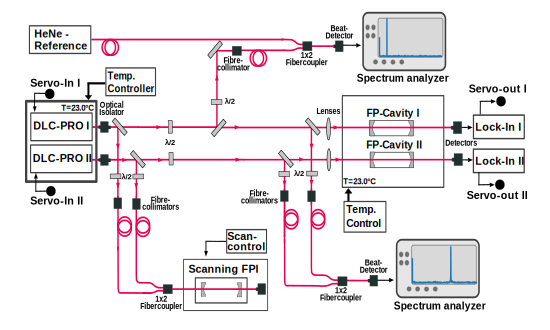
\includegraphics[width=\linewidth]{/Refraktometer_setup_drawing/experimental_setup_Refractometer}
	\caption{Shown is the refractometry-based experimental setup with all relevant optical and electronic devices.}
	\label{fig:experimental_setup_Refractometer}
\end{figure}
\noindent
The resonator to which the \textbf{reference Laser} (DLC-PRO I) is locked to will be called \textbf{reference resonator}. This resonator (FP-Cavity I) is constantly evacuated during all measurements. Locking the reference diode Laser to the evacuated cavity, stabilizes the output frequency of the Laser to the frequency of the respective, chosen TEM$_{00}$ of the cavity. This provides a great short therm frequency reference for the measurement Laser (DLC-PRO II), since the reference resonator has a high finesse (1000 to 10000 depending on the resonator used) and is is mostly influenced by external temperature fluctuations, which can result in long term drifts of the emission frequency. These short therm drifts can be visualized by measuring the beat between the stabilized HeNe-Laser and the reference Laser. This is achived by combining the two Lasers with a 2x1 fibre coupler and then measuring the beatsignal between the two with a beat detector and spectrum analyzer.\\\\
\noindent
The \textbf{measurement Laser} (DLC-PRO II) is another identical diode Laser, which is phase-locked to the \textbf{measurement Fabry-Pérot resonator} (FP-Cavity II). This, second resonator is filled with the measurement gas of choice for refractivity measurements. The refractivity is proportional to the change in beat frequency between the measurement and reference Laser and the beat frequency between the two lasers is observed on a beat detector after combining them with a 2x1 Fiber-coupler before the detector.\\\\
\noindent
The absolute frequency of the HeNe-Laser is known from the theoretical hyper-fine structure of the spectrum and provides a traceable absolute frequency reference for the two diode Lasers via the two simultaneous \textbf{beat measurements}. However, the bandwidth of the \textbf{beat detector} is limited to 3 GHz, which means that beat signals between the Lasers, that are larger than \mbox{3 GHz}, can not be detected. Since the two diode Laser have an extensive frequency tuning range it is required to adjust the Laser current and voltage so that the emission frequencies of the two diode Laser are within a detectable range of: $<3$ GHz to the HeNe-Laser. This pre-adjustment of the Lasers is done by using a wavemeter (High-Finesse: WS-5) which is used to measure the emission frequency of the Laser. The Laser current, voltage, grating-angle and temperature are adjusted until the emission frequency of the diode Lasers are aligned with the HeNe reference. \\\\
\noindent
Diode Lasers, especially at 633 nm, are vulnerable to switch abruptly to multi-mode operation. This can occur due to temperature changes or other external effects and results in the diode laser emitting more than one frequency at a time. However, for a refractometer a constant single mode operation is required to preserve the traceability of the laser frequencies and the beat measurements. To ensure that the Lasers are single mode at the chosen Laser configuration of: Laser- temperature, -current and -voltage, a \textbf{Scanning Fabry-Pérot} (Thorlabs: SA200-5B) is used. Both, the reference and the measurement Laser are coupled into the same Fabry-Pérot Interferrometer (FPI) and the transmission of the FPI is monitored on a detector connected directly to the cavity. If the Laser abruptly switches to multi-mode operation during a measurement, it can be observed on the FPI-detector immediately since additional transmission peaks will become visible in the transmission spectrum.\\\\
\noindent
To avoid external environmental influences, the two diode Lasers are integrated in a \textbf{temperature controlled} and vibration resistant enclosure. The enclosure consists of a Styrodur box with an integrated Peltier element which is set to stabilize the internal temperature to \mbox{23.0 $^{\circ}$C}. The FP-Cavities (FP-Cavity I and II) can be integrated into a water-cooled aluminum vacuum chamber, which is connected to a precision calibration bath (CIK: Kambic) with a temperature stability of 1 mk. The vacuum chamber itself is integrated into a multi-layer Sytrodur box, where each Layer contains water-cooled radiators to further stabilize the environmental temperature effects. The radiators are connected to water cooled bath (PolyScience: Mode: AP15R) and operate at \mbox{23.0 $^{\circ}$C}.\\\\
\noindent
As stated earlier, a unique feature is the \textbf{dichroic coating} of two of the available resonators. Those allow for simultaneous measurements at 1550 and 633 nm. As a \textbf{1550 nm Laser} source two identical fiber Lasers (NKT photonics: Koheras ADJUSTIK X15) were used. They are not shown in Figure \ref{fig:experimental_setup_Refractometer} intentionally, to provide a simplistic overview of the basic operating principle. For measurements however, the two fiber Lasers are spatially overlapped with the diode Lasers and separated again after the measurement and reference resonator respectively. The spatial separation is required to guide the individual lasers onto their respective wavelength-sensitive detectors. The separation is achieved with optical filters that transmit 633 nm and reflect \mbox{1550 nm} light and two additional \mbox{1550 nm} detectors for Laser-locking of the fiber-Lasers.
\newpage
\subsection{Vacuum system}
The vacuum system shown in this section is required to supply the measurement cavity with a pure measurement gas, a flexible pressure modulation as well as a traceable pressure reference for the refractivity measurements. 
Figure \ref{fig:experimental_setup_Refractometer_vauum_system} shows all the vacuum components used to construct the refractometry based pressure standard. The Fabry-Pérot Cavity I is again the reference cavity and the FP-Cavity II the measurement cavity. \\\\
\noindent
The \textbf{gas supply} for the measurement cavity is realized with a pure gas bottle of either: Nitrogen, Argon or Helium with the highest possible purity (between 5.0 and 7.0). The measurement gas then has to pass through an additional \textbf{sintered metal filter}, which further purifies the gas. A \textbf{Mass Flow Controller (MFC)} with an integrated electric valve and a maximum flow rate of \mbox{5 sccm} (standard cubic centimeter per minute) is used to control the gas flow into the system and the measurement cavity respectively. Before any measurement or after switching gas bottles, the vacuum system up to the Mass flow controller is flushed with the measurement gas several times. This is done by filling the tubing with the respective gas and evacuating it afterwards with the connected oil-free \textbf{Scroll pump}. Flushing the system with gas removes potential impurities in the tubing after switching bottles. \\\\
\noindent
For the evacuation of the system an additional set of a \textbf{turbomolecular pump} and a scroll pump can be used. All vacuum tubing is made of full metal materials and compatible with ultra-high-vacuum conditions.  \\\\

\begin{figure}[H]
	\centering
	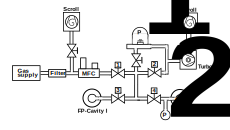
\includegraphics[width=\linewidth]{/Refraktometer_setup_drawing/experimental_setup_Refractometer_vauum_system}
	\caption{Shown are all thr required vacuum components used for the optical refractometer.}
	\label{fig:experimental_setup_Refractometer_vauum_system}
\end{figure}
\newpage
\noindent
A set of four \textbf{pneumatic valves} are used to control the gas flow through the vacuum system, they are labeled from 1 to 4. With open valves 2 and 3, the reference FP-Cavity-I can be evacuated. Additionally opening valve 4, allows for the simultaneous evacuation of the measurement cavity (FP-Cavity-II).\\\\
\noindent
During a measurement, the gas pressure inside the measurement cavity is modulated by opening valve 1 and setting the Mass-Flow-Controller to the desired gas-flow rate. During a measurement the pneumatic valve to the reference cavity (valve 3) is generally closed, so that the resonator remains constantly evacuated and provides a stable frequency reference. However, valve 2 remains open during a measurement so that one has an equilibrium between gas flow in and out of the system. Depending on how far the needle valve of the MFC is opened one can modulate the total pressure inside the system freely. Pneumatic valves are chosen intentionally, since they do not introduce any heat (though electrical heating) inside of the temperature controlled environment of the two resonators. \\\\
\noindent
To ensure SI-traceable refractivity measurements, several different pressure sensors can be used to assess the gas pressures. A set of three calibrated \textbf{resonant silicon gauges} (RSG made by WIKA, labeled as "\textbf{P2}" in Figure \ref{fig:experimental_setup_Refractometer_vauum_system}) are directly connected to the measurement chamber and are used to assess the total pressure within the measurement resonator. Additionally a calibrated \textbf{piston gauge} (labeled as "\textbf{P1}") can be utilized for setting the pressure in the system and performing directly traceable refractivity measurements.
\section{Resonator choice}
The heart of every Fabry Pérot based refractometer is the resonator, which is to be filled with measurement gas of choice. Generally speaking each resonator, used for FP-based refractometry, consists of a spacer material with a fixed length $l$ and a pair of mirrors which are contacted to the planar end surfaces of the spacer material. The choice of spacer material has a significant influence on the performance of the system and how the cavity reacts to environmental influences like temperature fluctuations or gas modulation. Often times, glass materials like: Zerodur, Ultra-low-expansion(ULE)-glass or Clearceram are used. The have the benefit of being polishable and allow for direct optical contact bonding of the mirror substrate with the spacer material, which does not require glues or binders. In many cases the mirror substrate can be fabricated from the same material as the spacer to create a solid bond between spacer and mirror after optical contacting. The three listed spacer materials also have the benefit of having a zero-crossing of the thermal expansion coefficient ($\alpha$) close to room temperature, which is the most common operating temperature in optical laboratories. In the case of Zerodur the thermal expansion coefficient is as low as : $10^{-6}/K$. Since the thermal expansion determines how much the size of the material changes due to temperature changes:
\begin{align}
	\frac{\Delta L}{L_0} = \alpha \Delta T
\end{align}
it becomes an important property when designing length sensitive Fabry Pérot refractometers. One disadvantage glass materials is their relatively high out gassing rate for Helium, which is a common calibration gas. Especially ULE-glass is know for taking up Helium rapidly when its is exposed to a Helium atmosphere and then slowly releasing the gas over time again. This characteristic of ULE (and other glasses), can result in unwanted long term drifts of the overall resonator length and require constant re-alibration.\\\\
An alternative to glass materials are metals, like stainless steel or Invar (a nickel iron alloy). These spacer materials typically have very low out gassing rates, which is one reason why they are commonly used for other vacuum applications. The trade off with stainless steel or Invar spacers is however, that the mirrors cannot be optically contacted or glued to the spacer material directly. Instead they the have to be mechanically pressed against the spacer and secured in place. Due to the high mechanical forces required to create a leak tight seal between the metal spacer and the mirrors, it is not uncommon to damage the mirror substrates during the process.\\\\
Figure \ref{fig:Different_resonatrors} shows three different resonators used by the National Metrology Institutes participating in the QuantumPascal project. A variety of different spacer materials, mirror substrates and cavity designs have been tested during the project period. 
\begin{figure}[H]
	\centering 
	\includegraphics[width=0.99\linewidth]{/Measurements_REF/Resonators/Different_resonatrors}
	\caption{A and B: Zerodur resonator used at the LNE-CNAM in france. A) shows the copper enclosure used for thermal stabilization of the Zerodur cavity. C) Invar based Fabry Pérot cavity design used by the PTB and the Umea university in sweden.}
	\label{fig:Different_resonatrors}
\end{figure}
\noindent
Within this thesis, glass based spacer materials where investigated for their out gassing behavior with the intend to characterize potential long term drifts and design guides for optimal resonator design with regards to FP- based refractometry. For refractivity measurements, an initial Zerodur based dual cavity system was used and later upgraded to an invar based resonator with a dichroic set of mirrors.
\subsection{Measurement of the coefficient of thermal expansion (CTE)}
The coefficient of thermal expansion (CTE) is a material property that is especially relevant when working with FP-based refractometers. The CTE of the spacer material of the resonator determines how sensitive the system is to temperature fluctuations and what quality of a thermal insulation is required to reach the target uncertainty of the refractometer. The temperature induced length change of the spacer material:
\begin{align}
	\frac{\Delta L}{L_0} = \alpha(T) \Delta T \approx \frac{\Delta f}{f_0}
	\label{eq:CTE}
\end{align}
depends on the coefficient of thermal expansion, $\alpha$ and the temperature change $\Delta T$. The CTE is a temperature dependent property but can be approximated as a constant value for a small temperature range if one wants to approximate the order of magnitude with an experimental approach. The change in cavity lengths can, in the case of a FP-based refractometer, be assessed with a beat measurement between the measurement- and a reference-Laser. \\\\
The CTE of the Invar based single cavity resonator was experimentally approximated with the setup shown in section \ref{sec:refractometer_setup}. The Zerodur resonator was used as a reference resonator and the Invar cavity was utilized for the CTE measurements. However, both resonators were constantly evacuated during the complete measurement campaign to eliminate pressure induced fluctuations of the beat signal. \\\\
To determine the CTE of Invar, the beat between the locked reference and measurement Laser were detected over time, while the temperature of the measurement cavity was modulated. The beat between the two laser fields is assessed with a beat detector and a spectrum analyzer, that can track any changes in beat frequency. Both, the reference and the measurement Laser are locked to the first TEM$_{00}$-mode of their respective resonators with a digital, FPGA based locking module using the LOCK-IN technique. The measurement resonator is positioned inside of multi-layer, thermally insulated box where the temperature is stabilized using a calibration water bath in combination with multiple water cooled radiators. The reference resonator was positioned in an outer layer of the thermally insulated box, so that a constant operating temperature and passive shielding from room temperature fluctuations could be ensured. \\\\
The temperature induced change in beat signal is proportional to the CTE as long as the system is free of other environmental influences like pressure modulations (which is guaranteed due to evacuation of the system). To introduce a temperature increase of the system, the measurement resonator temperature was modulated by programming the calibration bath to increase and decrease the bath temperature periodically. The starting temperature was chosen to be XX, so that it is similar to room temperature and was then step wise increased by 0.2 K and decreased again to the starting temperature. After increasing the temperature by 0.2 K, the system was given several hours time to stabilize its temperature before another step wise increase had been initiated. Figure \ref{label} shows the periodic modulation of the measurement-resonators temperature, which was induced by modulating the calibration baths temperature. One can also see the temperature of the reference resonator, which is indirectly modulated, although it is thermally and spatially shielded from the water cooled radiators (but not sufficiently). This results in a periodic and unwanted modulation of the reference Laser frequency, that will later be discussed in greater detail.\\\\
During the temperature modulation process, the beat signal was detected and Figure \ref{label} shows the beat signal between the two Laser fields for the same time period during which the temperature of the measurement resonator was modulated. The beat shows a similar modulation as the temperature measurement but is distorted by the indirect modulation of the reference resonator temperature due to insufficient thermal shielding. The beat signal is therefor not directly proportional to the initiated temperature modulation, since the reference frequency is also periodically changed.\\\\
Assuming that the CTE is constant for the small temperature range observed, one can approximate $\alpha$ as constant and extract it from the beat measurement. Therefore, the change in beat frequency, due to the temperature increase of 0.2 K, was extracted from Figure \ref{label} for each step of the periodic temperature modulation. The obtained values for $\Delta f$ where then averaged and the standard deviation was calculated to:
 \begin{align}
 	\Delta f^{T\rightarrow T \pm 0.2K} = 86.5 \ \text{MHz} \pm 10 \ \text{MHz}
 \end{align}
The large standard deviation is due to the unwanted temperature modulation of the reference resonator and therefore the reference Laser frequency. The approximated CTE of Invar can then be calculated using equation \ref{eq:CTE} :
  \begin{align}
 	\alpha=\frac{86.5 \text{ MHz}}{200 \text{ THz} \cdot 0.2 \text{ K}} = 2.1\cdot 10^{-6} / \text{K}
 \end{align}
where $f_0=200$ THz is the operating frequency of the utilized 1550 nm Lasers. \\\\
One can now simulate the change in beat frequency due to the "constant" CTE of the Invar and subtract it from the measurement data in Figure \ref{label} to investigate the measurement residuals. Figure \ref{label} shows the raw data after subtracting the temperature induced change of the frequency of the measurement Laser from the measurement. What remains is the change in beat signal that was introduced by the unwanted frequency modulation of the reference Laser due to insufficient temperature shielding/ stabilization of the reference resonator. By comparing the measurement residuals with the temperature of the reference Laser (shown in Figure \ref{label}) one can observe that both signals have the same periodicity. 
\section{GAMOR method}
The Gas modulation refractometry (GAMOR) method is a gas refractivity measurement technique, developed and popularized by the swedish metrology research groups from the RISE (Research Institute of Sweden) and the Umea university \cite{Axner-2021}. \\\\
For Fabry-Pérot based measurement techniques of the refractivity, the  measurement gas is introduced into the cavity, which results in a shift of the resonator mode frequencies. If a (measurement) Laser is phase-locked to one of the resonator modes, this shift can be converted to a shift in Laser frequency. By comparing the frequency of the measurement Laser with the frequency of a second (reference) Laser that is phase-locked to an evacuated reference Fabry-Pérot Cavity, one can detect a change in beat frequency between the two Lasers. The change in refractivity can thereby be directly linked down to a simple beat measurement on a photodetector that combines the two Laser fields.\\\\
For a Laser that is locked to a cavity mode of a fully evacuated resonator, its unmodified frequency $\nu_m^{(0)}$ is given as:
\begin{align}
	\nu_m^{(0)}= \frac{q_m^{(0)}c}{2L_m^{(0)}}
\end{align}
where $q_m^{(0)}$ is the longitudinal resonator mode with mode number $m$ and $L_m^{(0)}$ the empty resonator length. If gas is let into the resonator additional effects that modify the mode frequency and cavity length have to be accounted for and the gas filled resonator mode frequency $\nu_m^{(g)}$ is given as:
\begin{align}
	\nu_m^{(g)}= \frac{\left( q_m^{(0)} +\Delta q_m^{0\rightarrow g} \right) c}{2 n_g\left( L_m^{(0)} + \delta L_m^{0\rightarrow g} \right)} 
	= \nu_m^{(0)} \left( \frac{1+\frac{\Delta q_m^{0\rightarrow g} }{ q_m^{(0)}}}{n_g\left(1+ \frac{\delta L_m^{0\rightarrow g}}{L_m^{(0)}} \right)}\right)
	= \nu_m^{(0)} \left( \frac{1+\Delta \bar{q}_m^{0\rightarrow g} }{n_g\left(1+ \delta \bar{L}_m^{0\rightarrow g} \right)}\right)
\end{align}
where $n_g$ is the refractive index of the measurement gas, $\delta L^{0\rightarrow g}$ is the change in cavity lengths by pressure induced deformation and $\Delta q^{0\rightarrow g} $ accounts for mode jumps during the introduction of gas into the cavity. In the last step the equation was simplified by introducing relative mode- and lengths-change variables: $\Delta \bar{q}_m^{0\rightarrow g}$ and $\delta\bar{L}_m^{0\rightarrow g}$.\\\\
\noindent
For a beat measurement between the measurement Laser with the frequency: $\nu_m^{(g)}$ and the reference Laser with the frequency:
\begin{align}
	\nu_r^{(0)}= \frac{q_r^{(0)}c}{2L_r^{(0)}}
\end{align}
the two Laser fields are spatially overlapped and a RF signal, between 0 and 4 GHz, can detected on a photodetector. The respective beat signal: $f_{(0,g)}$ for an evacuated reference cavity and a gas filled measurement cavity, then becomes: 
\begin{align}
	f_{(0,g)}= \nu_r^{(0)}- \nu_m^{(g)}=\nu_r^{(0)} - \nu_m^{(0)} \left( \frac{1+\Delta \bar{q}_m^{0\rightarrow g} }{n_g\left(1+ \delta \bar{L}_m^{0\rightarrow g} \right)}\right)
\end{align}
\noindent
Although the basic operating principle of a FP-based refractometer seems simple initially, in praxis it comes with many experimental challenges. One mayor challenge are system drifts of various kinds, that influence the Fabry-Pérot cavity over the measurement period or longer time scales. These drifts usually alternate the lengths of the cavity through different physical effects like: temperature fluctuations, out gassing of the cavity spacer materials or gas leaks in the vacuum system. A change in cavity lengths or increasing gas impurities result in a change of resonator mode frequency, that is not related to a change of measurement gas refractivity. \\\\
The GAMOR methodology is able to eliminate linear drifts by periodically measuring the gas refractivity at a given pressure P with a follow up measurement of the base line at a \mbox{pressure P $\approx$ 0}, at an evacuated state of the measurement resonator. Constantly tracking the baseline drift of the resonator allows for a simple correction by interpolating the zero measurements. Since the drifts are linear, on a short time scale, one can use the interpolated correction of the baseline to also correct the actual refractivity measurements that were carried out in between the baseline measurements. \\\\
\noindent
Figure \ref{fig:GAMOR_Cycle_before_correction} shows an example of two consecutive GAMOR cycles, were the measured beat signal between a 1550 nm, phase locked reference- and measurement-Laser is plotted against time. Each GAMOR cycle starts and ends with a baseline measurement to track baseline drifts, which in this case are introduced by temperature fluctuations of the system, as can be seen in the respective resonator-temperature profile at the bottom of Figure \ref{fig:GAMOR_Cycle_before_correction}. The temperature was observed during the beat measurements with an SPRT that was integrated into the measurement cavity. After the zero measurements, several refractivity measurements were performed at different pressures, by introducing or removing Nitrogen gas into the measurement resonator through an automated needle valve. The modulation of the gas pressure inside the measurement resonator results in the expected shift in the beat signal between the reference- and measurement-Laser.
\begin{figure}[H]
		\centering 
		\includegraphics[width=0.85\linewidth]{/Measurements_REF/GAMOR/GAMOR_Cycle_before_correction_mit_temp}
		\caption{\textbf{Top}: Exemplaric GAMOR cycle with a baseline drift  of the beat signal, due to temperature fluctuations inside the measurement resonator. \textbf{Bottom}: Temperature change within the measurement resonator during the measurement time period.}
		\label{fig:GAMOR_Cycle_before_correction}
\end{figure}
\noindent
The interpolated baseline drift can then be used to correct the beat signal for drifts, in this case introduced by cooling down the measurement resonator by 0.2 K over a time period of 90 minutes. Figure \ref{fig:GAMOR_Cycle_after_correction} shows a comparison between the corrected beat-signal-measurement and a pressure measurement that was performed simultaneously with a group standard of three calibrated resonant silicon gauges. The modulation of the Nitrogen pressure inside the resonator directly results in a change in gas refractivity that can be detected with the refractometer and both, the beat signal and cavity gas pressure are proportional to each other.
\begin{figure}[H]
	\centering
	\includegraphics[width=\linewidth]{/Measurements_REF/GAMOR/GAMOR_Cycle_RSG_pressure_and_beat}
	\caption{\textbf{Left}: Corrected beat signal during a measurement cycle.
	\textbf{Right}: Measurement of the Nitrogen pressure inside the measurement-resonator.}
	\label{fig:GAMOR_Cycle_after_correction}
\end{figure}
\section{Free-Spectral-Range of the Invar resonator}
The free-spectral-range (FSR) of a resonator is an important property that can be determined experimentally with different approaches.
It is defined as: 
\begin{align}
	\Delta \nu = \frac{c}{2 n L}
\end{align}
where $\Delta \nu$ is the frequency difference between two consecutive TEM$_{00}$ modes of the cavity, $L$ is the length of the resonator and $n$ is the refractive index of the investigated gas. \\\\
With respect to FP-based refractometry, precise knowledge of the FSR is required to determine the change in beat frequency during a refractivity measurement. When filling the measurement resonator of a dual Fabry Pérot cavity with gas, the beat frequency between the detected reference- and measurement-Laser fields is given by:
\begin{align}
	f_{0,g} =\nu_{r}^{0}-\nu_{m}^{g}= \nu_{r}^{0}-\nu_{m}^{0} \left(\frac{1+\Delta q_m^{0 \rightarrow g}}{n_g(1+\delta L^{0 \rightarrow g})}    \right)
\end{align}
as it was shown in the previous section. Whenever the relative mode number $\Delta q_m^{0 \rightarrow g}$ changes by one, due to the introduction of gas into the system, the beat frequency changes by the exact value of the FSR of the measurement resonator.
It is possible to determine the FSR of any resonator by measuring its length or by directly determining the frequency difference between two consecutive TEM$_{00}$-modes of the cavity. Both methods are valid but generally frequency measurements can be carried out with greater precision and are therefore often times preferred. \\\\
To determine the FSR, the 1550 nm measurement Laser is phase locked to the first TEM$_{00}$- mode of the measurement resonator, same as the reference Laser with its respective cavity. An initial beat measurement is carried out between the two Laser fields, while both cavities are positioned in th same temperature controlled environment. The lock of the measurement laser is then released from the first TEM$_{00}$-mode and is instead locked to the next adjacent TEM$_{00}$-mode. This can be achieved by adjusting the operating-voltage, -current or -temperature of the measurement Laser, so that it emission frequency is closer to the frequency of the second TEM$_{00}$-mode of the resonator. The lock can then be re-engaged and the Laser emission frequency is stabilized to the respective frequency of the adjacent resonator mode. \\\\
The lock of the reference Laser remains unchanged and a second beat measurement between the two Laser fields is performed. For stable environmental conditions, the detected change in beat frequency between the two system configuration is equal to the FSR of the measurement resonator. Figure \ref{fig:FSR} shows the beat measurement between the two laser fields of the 1550 nm Laser systems before and after changing the lock of the measurement cavity mode by $\Delta q_m^{0 \rightarrow 1}$. 
\begin{figure}[H]
	\centering
	\includegraphics[width=0.99\textwidth]{/Measurements_REF/FSR/FSR-measurement}
	\caption{.}
	\label{fig:FSR}
\end{figure}
\noindent
To improve the measurement uncertainty of the FSR, the described lock and re-lock of the measurement Laser was repeated several times. The beat signal for each system configuration, was measured for ten minutes and the signal was then averaged over time to account for eventual temperature instabilities during the ten minute period. Two consecutive measurements can then be compared to each other to determine the FSR of the resonator. The beat signal, where both Laser are locked to their respective first TEM$_{00}$- modes, are around 1.24 GHz. While the beat signal measurement of the second configuration yields around 1.16 GHz.
\\\\ By adjusting the measurement Lasers operating Voltage, to lock it to the second TEM$_{00}$, the beat signal reaches zero and increases again (up to a value of 1.16 GHz). Resulting in an initial estimated FSR value of: 2.4 GHz. Since the beat signal "crossed" zero both configurations react anti proportional to the temperature fluctuations during the measurement. Fluctuations of the temperature where measured with an SPRT and could be corrected for. Within the raw measurement data, in Figure \ref{fig:FSR}, they are visible as an overall trend that results in a slow change of the detected beat frequency, which is in the order of 1.5 MHz per hour.\\\\
The results of the individual FSR-measurements where then averaged again and the FSR of the measurement cavity could be determined as:
\begin{align}
	\Delta \nu_{meas}= 2.407 \text{ GHz} \pm xxxx
\end{align}
\section{Temperature and pressure assessment}
FP-based refractometers are highly sensitive to temperature fluctuations of the gas, which potentially allows them to be used as thermometers as well, if the respective gas pressure is known instead. The temperature stability requirements during a gas density measurement are therefore high and often times require a multi layered temperature stabilization of the system. During this thesis the refractometer could be integrated into a water cooled, aluminum based vacuum chamber which was connected to a calibration bath with a temperature stability of 1 mk (CIK: Kambic). The vacuum chamber was integrated into a multilayered, temperature controlled enclosure made of Styrodur. Radiators, that are connected to the same calibration bath are used to control the air temperature of the enclosure to the same value as the vacuum chamber.  \\\\  
During a refractometry measurement, the gas temperature is assessed with two 25 Ohm standard platinum resistance thermometers (SPRT) which are connected to a measurement bridge (Isotech:MircoK 70) and a reference resistor. Depending on the resonator used, the SPRTS are either directly integrated into the Cavity itself (inserted into a drilled bore) or in direct contact with the cavity. Over a period of 2 years, the SPRTs were calibrated three times against the water triple point and the Gallium melting point in the temperature laboratory of the PTB. During the calibration, the same measurement bridge was used, which compensates for the self heating of the SPRT-sensors which require an operating current of 1 mA. The resistance of the SPRT is assessed with a four wire measurement and then internally compared to the reference resistor. The reference resistor itself is integrated into a temperature controlled box which operates at \mbox{23 $^{\circ}$C}. With the help of the calibration certificate the measured resistances of the SPRTs can then be converted into temperatures. Figure \ref{fig:/PTB_Temperature_SPRTs} shows the stability of the calibration bath that is used for thermostatisation of the resonator and experimental enclosure. The temperature was assessed with the two SPRTs over a time period of 140 hours. 
\begin{figure}[H]
	\centering
	\includegraphics[width=\linewidth]{/Measurements_REF/Temperature_stability/PTB_Temperature_SPRTs}
	\caption{Temperature stability of the calibration bath assessed with two calibrated SPRTs labeled: 347 and 348. Shown is the respective measurement data together with a running mean over 100 seconds. At the bottom, the temperature difference $\Delta T$ between the two sensors is shown. For the running mean it is in the order of $4\cdot 10^{-5}$ K with a standard deviation of  $7\cdot 10^{-6}$ K. }
	\label{fig:/PTB_Temperature_SPRTs}
\end{figure}
\noindent
If a gas \textbf{pressure} assessment was required for a refractivity measurement, a group standard of three identical resonant silicon gauges (RSG) could be used for pressure ranges from 1 Pa to \mbox{100 kPa}. Over the course of this thesis the sensors were calibrated three times against the static expansion system 3 of the vacuum metrology working group at the PTB. Alternatively, two calibrated piston gauges could be used to set the measurement pressure in the cavities between \mbox{1 kPa} and \mbox{100 kPa}.
\newpage
\section{Refractivities of Helium, Nitrogen and Argon}
The refractivity of a gas is not only pressure dependent, which allows for the design and construction of FP-based pressure standards, but it is also frequency dependent. A Fabry-Pérot cavity with dichroic mirrors can therefore be used to investigate the frequency dependence of the refractivity by performing the same refractivity measurements simultaneously at two (or more) Laser wavelengths e.g 633 and 1550 nm.\\\\
During this thesis, the refractivities of the thre gases: Helium, Argon and Nitrogen were investigated. \\\\
\textbf{Helium} is chosen as a calibration gas for the refractivity measurements since it is one of the few gases where precise calculations of gas parameters, like the refractivity and density virials, can be carried out in a reasonable time frame. This is due to its molecular properties as a noble gas and low number of atoms involved. \textbf{Nitrogen} is chosen since almost all industrial pressure sensors are calibrated with Nitrogen gas at national metrology institutes and it is one of the most abundantly available gases. Theoretical calculations for gas parameters of \textbf{Argon} are more challenging but comparisons with experimental resesarch can improve the overall understanding and future calculations. Argon is therefore chosen as a third gas. \\\\
To investigate and measure the refractivity of the three aforementioned gases, the dual cavity Fabry-Pérot system was used (see Figure \ref{fig:experimental_setup_Refractometer} of the experimental setup section)s. The dichroic \textbf{Invar resonator} was chosen as a measurement resonator, while the Zerodur cavity was used as a reference. Two sets of two Lasers were used to investigate the frequency dependence of the individual gas refractivities, where one \textbf{set of Lasers} operates at 633 nm and the other one at 1550 nm. Experimentally, the two measurement Lasers were spatially overlapped and separated using selective optical filters. The filters are reflective for 633 nm and transmit 1550 nm laser light. Both wavelengths were then sent through the Invar resonator and locked to a TEM$_{00}$-mode of the cavity. The beat signals to their individual reference Lasers, at 633 and 1550 nm respectively, was detected with two sets of beat detectors. Any change in beat frequency was visualized and tracked with a spectrum analyzer. The pressure in the measurement resonator was controlled using a fully automatic needle valve. If the pressure is modulated adequately, one can count the TEM$_{00}$-modes and obtain the required change in modenumber $\Delta q^{P_1 \rightarrow P_2}$ in between measurements at the arbitrary set pressures $P_1$ and $P_2$.\\\\
At all points during the measurement, the reference cavity was fully evacuated using a turbomelecular pump. The pressure in the measurement cavity was modulated using the GAMOR methodology and tracked with a set of three, calibrated resonant silicon gauges. The gas pressure in the resonator was step wise modulated between 0.1 and 360 Pa. To avoid cross contamination and preserve the respective gas purity, measurements with different gases were carried out successively. In between measurements the \textbf{vacuum system} was fully evacuated and flushed several times with the new measurement gas to get rid of potential residual gases in the vacuum system and resonator.\\\\
The obtained change in beat frequency $\frac{\Delta \nu}{\nu_0} $ can then be used to determine the gas refractivity for the given pressure range via:
\begin{align}
	(n-1) &= \frac{\frac{\Delta_{\nu}}{\nu_0}+\frac{\Delta_q}{q_0}}{1-\frac{\Delta_{\nu}}{\nu_0} +\epsilon_m}
\end{align}
where $\epsilon_m$ is a deformation coefficient, the calculation of which is explained in more detail in the following chapter. Figure \ref{fig:refractivity_all_gases} illustrates the experimental results for all three gases and the two chosen Laser wavelengths.
\begin{figure}[H]
	\centering
	\includegraphics[width=\linewidth]{/Measurements_REF/Refractivity/refractivity_all_gases_1}
	\caption{Shown are the combined refractivity measurements for Helium, Argon and Nitrogen for a pressure range between 1 and 350 Pa. Measurements were performed simultaneously at two different wavelengths (633 and 1550 nm).}
	\label{fig:refractivity_all_gases}
\end{figure}
\noindent
The measurement effect for Helium is around 8 times smaller than that of Nitrogen and 7.1-times smaller than that of Argon. One can also observe the clear frequency dependence of the refractivity in the zoomed-in section of Figure \ref{fig:refractivity_all_gases}. The measured refractivity, at identical pressures but different Laser wavelengths, is always smaller for greater wavelengths. At 1 Pa, the fractions $\delta(n-1)=\frac{(n-1)_{1550 \text{ nm}}}{(n-1)_{633\text{ nm }}}$ are given as:
\begin{table}[H]
	\begin{center}
		\begin{tabular}{ llll }
			
			Gas : & Helium: & Argon: & Nitrogen\\
			\toprule
			$\frac{(n-1)_{1550 \text{ nm}}}{(n-1)_{633\text{ nm }}}$ : & 0.994   & 0.989 & 0.988\\
			\bottomrule
		\end{tabular}
	\end{center}
	\caption{Frequency dependence of the refractivity}
	\label{table:Frequency dependence of the refractivity}
\end{table}
\noindent
The measured refractivity can now be used to determine the gas density, if the one wants to utilize the refractometer as a pressure standard. By using the theoretical values for the refractivity virials: A and B, together with the density virial $B_{\rho}$ as shown in the theory part of this thesis:
\begin{align}
	\rho &= \frac{2(n-1)}{3A}\cdot \left(1-\frac{1+4B}{A^2}(n-1)\right)\\
	P&=RT\rho \left(1+\rho B_{\rho}\right)
\end{align}
It is however required to further analyze the system with respect to its pressure dependent deformation before it can be utilized as a pressure standard. The deformation results in a pressure dependent lengths change of the cavity that results in an additional measurement effect.
\section{Pressure induced cavity deformation}
Within the QuantumPascal project, many pressure standards are developed at the individual National metrology institutes (NMIs) of which many utilize external cavities. The resonators are either integrated directly into the measurement unit (e.g in the case of a refractometer or for cavity ring down spectroscopy) or function as a frequency reference for the Pound-Drever-Hall or Lock-In technique. A simple Fabry-Perot resonator consists of a spacer material and two mirrors, which are attached to the end surfaces of the spacer substrate. The spacer ensures a constant distance between the mirrors and prevents them from tilting. The distance between the mirrors defines the standing wave that is formed inside the resonator and has to be well known for accurate measurements of the refractivity. The distance between the mirrors can deviate significantly due to enviromental influences such as temperature changes or mechanical deformations due to pressure. This cavity deformation can be accessed with finite element simulations, using commercial programs like COMSOL or ANSYS, for a given set of spacer and mirror materials.

\subsection{Deformation of a specific cavity with COMSOL}
As preparatory work to simulating the deformation of a cavity used for CRDS, the pressure dependent deformation of a Fabry-Perot resonator, designed by the LNE-Cnam (Laboratoire commun de métrologie), was investigated with the commercial program COMSOL. The examined resonator consists of a 100 mm long Zerodur spacer to which two fused-silica mirrors, with a diameter of 50 mm and a thickness of 15 mm, were optically contacted. The spacer material itself has an inner diameter of 34 mm and an outer diameter of 54 mm. The material properties of Zerodur and fused silica, which are needed to determine the mechanical deformation of the mirrors, are listed in table \ref{table:COMSOL-parameter-cavity-franzosen}. Figure \ref{fig:CNAM-cavity-3D} (a and b) show a 3D-model of the resonator and its symmetry planes. 
\noindent
\begin{table}[H]
	\begin{center}
		\begin{tabular}{ lll }
			
			\textbf{Material}: & \textbf{Zerodur} & \textbf{Fused Silica}\\
			\toprule
			Density (kg/m$^3$): & 2530  & 2195\\
			\midrule
			Poisson number:  & 0.240 &  0.155\\
			\midrule
			Thermal conductivity (W/ m K): & 1.46  & 1.25\\
			\midrule
			Youngs modulus (GPa): & 90.3  & 73.0\\
			\midrule
			Thermal expansion coef. (1/ K): & 2.00$\cdot 10^{-8}$  &5.55$\cdot 10^{-7}$\\
			\bottomrule
		\end{tabular}
	\end{center}
	\caption{Material properties of Zerodur and fused silica.}
	\label{table:COMSOL-parameter-cavity-franzosen}
\end{table}

\begin{figure}[h]
	
	\begin{subfigure}[t]{.45\textwidth}
		\centering
		\includegraphics[width=\linewidth]{/COMSOL-Cavity-Deformation/Plots/Grid-Cavity}
		\caption{3D-model of the resonator and mesh grid.\hfill}
	\end{subfigure}
	\hfill
	\begin{subfigure}[t]{.45\textwidth}
		\centering
		\includegraphics[width=\linewidth]{/COMSOL-Cavity-Deformation/Plots/Loslager-Cavity}
		\caption{Symmetry planes of the cavity.\hfill}
	\end{subfigure}
	
	\medskip
	\begin{subfigure}[t]{.45\textwidth}
		\centering
		\includegraphics[width=\linewidth]{/COMSOL-Cavity-Deformation/Plots/one-eigths-cavity}
		\caption{X-Y plane of the simplified 3D-model.\hfill}
	\end{subfigure}
	\hfill
	\begin{subfigure}[t]{.45\textwidth}
		\centering
		\includegraphics[width=\linewidth]{/COMSOL-Cavity-Deformation/Plots/one-eigths-cavity-y-z-plane}
		\caption{Y-Z plane of the simplified 3D-model.\hfill}
	\end{subfigure}
	
	\caption{Shown is the complete 3D-model of the simulated resonator (a), the three symmetry planes of the object (b), aswell as the simplified 3D-model which was used to minimize computation time (c and d).}
	\label{fig:CNAM-cavity-3D}
\end{figure}
\noindent
The 3D object was created within COMSOL using the linear elastic model and assuming that both materials are joined together, forming one solid object without a junction area. The 3D-model of the cavity is divided into small mesh elements with a user defined size. Depending on the size of these mesh elements, the simulation accuracy and computation time can be enhanced or decreased. For the first iteration of the simulation a minimal element size of $1.3 \cdot 10^{-3}$m and a maximum element size of $1.3 \cdot 10^{-5}$m were defined. In this configuration the resonator was separated into a total number of $190.000$ mesh elements. It is possible to reduce the required computation time further by utilizing the symmetry planes of the resonator. Since the cavity is symmetric around three planes, it is sufficient to simulate only $1/8$th of the object (see Figure \ref{fig:CNAM-cavity-3D} (c and d)) without losing any information. 
\newpage
\noindent
After the modeling process is complete one can apply a fixed force per area to all external surfaces of the resonator in order to estimate the pressure induced deformation with the finite element simulation. In the case of a refractometer the deformation of the mirrors along the z-axis (optical axis) is most important.  Fig.\ref{fig:Displacement-map} shows a displacement map of the spacer and mirror surfaces after a pressure of 1 Pa was applied to the system. The displacement of the materials increases quadratically from the center point of the mirror to the edges for the given pressure value. The absolute deformation of the mirror center is in the order of $-3 \cdot 10^{-13}$m. The relative length change of the complete resonator: $\frac{\delta L}{L} $ can be calculated and was determined to be: $-6.39 \cdot 10^{-12}$.
\begin{figure}[H]
	\centering
	\includegraphics[width=.75\linewidth,height=257px]{/COMSOL-Cavity-Deformation/Plots/Absolute_displacement_at_1Pa}
	\caption{Shown is the displacement of the X-Y-Plane in the direction of the optical pathway (z-axis). The surface includes the mirror and the spacer materials.}
	\label{fig:Displacement-map}
\end{figure}
\noindent
To determine the pressure dependent deformation, the simulation was repeated several times for additional pressure values in the range of 1 Pa to 1 kPa. As a reference point the center of the mirrors was chosen. The relative displacement of the center points is then plotted against the simulated pressure value (see Figure\ref{fig5a}). A linear correlation between the simulated pressure and the relative deformation can be observed and the corresponding fit function was determined to be:
\begin{equation}
	f(x)= (-6.39\cdot 10^{-12} \pm 3.9\cdot 10^{-22})\cdot x
\end{equation}\\ 
\newpage
\noindent
\begin{figure}[ht]
	\centering
	\includegraphics[width=0.9\linewidth]{/COMSOL-Cavity-Deformation/Plots/Pressure-dependant-deformation}
	\caption{Shown is the pressure dependent displacement of the central mirror-point along the optical axis.}
	\label{fig5a}
\end{figure}
\newpage
\noindent

\subsection{Experimental determination of the deformation}
The pressure induced deformation of a FP-cavity based refractometer is a highly specific to the respective system. It greatly depends on the cavity materials used, potential material defects, the contacting of the mirrors to the resonator and other environmental effects. A theoretical FEM simulation of a pressure induced deformation of the chosen system can therefore only ever be a rough approximation of the actual, physically observable deformation. For a refractometry based pressure standard it is therefore required to experimentally determine the deformation of the system to account for these highly specific effects and not to rely on a FEM-simulation. \\\\
The pressure induced deformation of the resonator can be determined experimentally with the so called: Two-gas-method and the following section will be used to illustrate the experimental approach of the method.\\\\
A FP based refractometer is used to perform two individual pressure measurements with Helium and Nitrogen. These two gases are chosen because their respective measurement effects (change in beat frequency due to pressure modulation) are different by almost one order of magnitude. The deformation of the cavity mirror however, is independent of the gas species and scales linear with pressure. This observation allows for a clever method to extract the deformation coefficient $\epsilon_m = \frac{\Delta L}{L_0}/(n-1)$, by comparing the two partial pressure measurements of Helium and Nitrogen with each other over a fixed  pressure range. \\\\
Additionally, Helium and Nitrogen are chosen as measurement gases because their refractivity and density virial coefficients can be theoretically calculated with the uncertainties required for a high precision refractometry based pressure standard. This allows for a comparison of the theoretically expected partial pressure values with the experimentally obtained result for gas pressure and gas density measurements. Since the cavity-length-deformation along the optical axis of the resonator scales linearly with pressure, one can obtain the deformation of the system by looking at the measurement residuals or rather the difference between theory and experiment.  \mbox{Figure \ref{fig:Measurement_residuals_refractometer}} shows a comparison of the (theoretical) set pressure and the difference: $\Delta P$ between the set pressure $P_{set}$ and the experimentally obtained pressure $P_{meas}$. If the measurement pressure is not corrected for the deformation of the system, a clear pressure dependent difference between theoretical and experimental pressure can be observed. \\\\
The difference $\Delta P$ increases linearly with pressure for both, Nitrogen and Helium. The deviation originates from the linear deformation of the cavity mirrors due to an increase in measurement pressure. However, the difference $\Delta P$ between the experimental and theoretical result are around 8 times higher for Helium than for Nitrogen, This is due to the measurement effect being 8 times stronger for Nitrogen than for Helium (see Figure \ref{fig:refractivity_all_gases}). As a result, the relative error for Helium is larger in comparison to Nitrogen, since the deformation has a greater relative effect for a smaller overall measurement effect.\\\\
\begin{figure}[h]
	\centering
	\includegraphics[width=0.9\linewidth]{/Measurements_REF/Deformation/Measurement_residuals_refractometer}
	\caption{Shown is the difference $\Delta P$ between the experimental and theoretical pressures with respect to the chosen set pressures. This was done for Helium (blue) and Nitrogen gas for set pressures between 0 and 350 Pa.}
	\label{fig:Measurement_residuals_refractometer}
\end{figure}\\\\
To obtain the experimentally determined gas density and pressure from the refractivity measurements shown in Figure \ref{fig:Measurement_residuals_refractometer} the following relations were used:
\begin{align}
	(n-1) &= \frac{\frac{\Delta_{\nu}}{\nu_0}+\frac{\Delta_q}{q_0}}{1-\frac{\Delta_{\nu}}{\nu_0} +\epsilon_m}\\
	\rho_{exp} &= \frac{2(n-1)}{3A}\cdot \left(1-\frac{1+4B}{A^2}(n-1)\right)\\
	P_{exp}&=RT\rho_{exp} \left(1+\rho_{exp} B_{\rho}\right)
\end{align}
with the refractivity virials $A$ and $B$, the density virial $B_{\rho}$, the change in beat frequency: $\frac{\Delta \nu}{\nu_0}$ and the mode number change: $\frac{\Delta q}{q_0}$. The deformation coefficient $\epsilon_m = \frac{\Delta L}{L_0}/(n-1)$ is unknown at this point and will be determined through the two-gas method.\\\\
The theoretical refractivity is determined from the chosen set-pressure and the resulting gas density as follows:
\begin{align}
	P_{set} &=\text{const.}\\
	\rho_{theo} &= \frac{\sqrt{\frac{4B_{\rho}P_{set}+RT}{RT}}-1}{2B_{\rho}}\\
	(n-1)_{theo}&= \frac{A^2-\sqrt{A^3\left(-6A^2\rho_{theo}+A-24B\rho_{theo}\right)}}{2A^2+4B}
\end{align}
To obtain the deformation of the resonator: $\epsilon_m = \frac{\Delta L}{L_0}/(n-1)$, the data from Figure \ref{fig:Measurement_residuals_refractometer} is fitted with a linear model for each individual gas. The respective slopes of the linear fits, named $k_{N_2}$ and $k_{He}$, are used to extract the deformation coefficient $\epsilon_m$ by comparing the two results with each other:
\begin{align}
	\epsilon_{m}(N_2)&=\frac{A_{He}}{A_{N_2}}\left( \frac{k_{He}-k_{N_2}}{1-\frac{A_{He}}{A_{N_2}}}  \right)\\
	\epsilon_{m}(He)&=\frac{k_{He}-k_{N_2}}{1-\frac{A_{He}}{A_{N_2}}}\\
	\frac{\Delta L}{L_0}&= \epsilon_{m} \cdot (n-1)
\end{align}
The following theoretically determined gas parameters were used for the calculation of $\frac{\Delta L}{L_0}$:
\begin{table}[H]
	\begin{center}
		\begin{tabular}{ lll }
			
			Gas property: & Helium: & Nitrogen:\\
			\toprule
			Refractivity virial (A) : & $0.52025865 \cdot 10^{-6}$   & $4.446107\cdot 10^{-6}$ \\
			\midrule
		    Refractivity virial (B):  &  $15.239 \cdot 10^{-12}$ & $0.81 \cdot 10^{-12}$\\
			\midrule
			Density virial ($B_{\rho}$):  &  $11.835 \cdot 10^{-6}$ & $-5.34 \cdot 10^{-6}$\\
			\midrule
			Gas temperature in Kelvin:  &  296.15 & 296.15\\
			\bottomrule
		\end{tabular}
	\end{center}
	\caption{Gas properties of Helium and Nitrogen}
	\label{table:gas_properties_Helium_Nitrogen}
\end{table}
\noindent
and together with the previously obtained mode number shift and Free-Spectral-Range of the cavity, the experimentally determined deformation of the resonator yields: 
\begin{align}
	\frac{\Delta L}{L_0}&=  7.47 \cdot 10^{-12} m/Pa
\end{align}
For all future pressure measurements with the given system this experimentally determined deformation factor can be utilized to correct the respective partial pressure measurements. The correction factor can be applied to all partial pressure measurements, independent of the gas species.

\section{Temperature effects: PV-work}

\begin{figure}[ht]
	\centering
	\includegraphics[width=0.8\linewidth]{/Measurements_REF/PV-work/PV_work_Fig_3}
	\caption{.}
	\label{fig:PV_work_Fig_3}
\end{figure}
aaaa
\newpage
\noindent
\begin{figure}[ht]
	\centering
	\includegraphics[width=0.9\linewidth]{/Measurements_REF/PV-work/PV_work_Fig_4}
	\caption{.}
	\label{fig:PV_work_Fig_4}
\end{figure}
aaa
\newpage
\noindent
\begin{figure}[ht]
	\centering
	\includegraphics[width=0.9\linewidth]{/Measurements_REF/PV-work/PV_work_Fig_5}
	\caption{.}
	\label{fig:PV_work_Fig_5}
\end{figure}
aaa
\newpage
\section{Ring comparison}
Circular comparisons are a tool in metrology to assess the repeatability, longtime performance and measurement uncertainty of pressure standards and other unit defining standards. The comparisons are generally performed internationally between multiple national metrology institutes. One, often times transportable, standard is chosen and directly compared to multiple other stationary standards which are present in the individual NMI's. A pre-defined measurement routine is agreed upon, and the staff members at each institute performs the respective measurements independently. Ultimately, the data is gathered and one can asses if the measurements agree with each other within the set boundaries.\\\\
Within the QuantumPascal project, the National metrology institute of Sweden together with the Umea university designed and built a transportable optical pressure standard. To assess the performance of this newly developed, state of the art optical standard a circular comparison was performed. Therefore the transportable optical standard was shipped to all participating NMI's and compared to the local, calibrated piston gauges of the pressure and vacuum laboratories. The combined data was then published in a project report \cite{label} and open access journal \cite{label}. \\\\
The operating principle of the transportable, optical pressure standard is based on a dual Fabry-Pérot resonator made of Invar combined with a mirror coating for a single wavelengths at 1550 nm. The GAMOR methodology was implemented and the system is able to assess vacuum from 1 Pa up to atmospheric pressure. To accommodate the refractometer for transportation, it was built to fit into a compact 19 inch rack with a 60x60 cm foot print at a height of 120 cm.
Figure \ref{fig:TOP} shows a picture of the transportable optical pressure standard (TOP) and \mbox{Figure \ref{fig:TOP_piston_gauge}} illustrates the measurement procedure when it is connected to a pressure balance at a NMI.\\\\
\begin{figure}[h]
	\begin{subfigure}[t]{.49\textwidth}
		\centering
		\includegraphics[width=\linewidth]{/Measurements_REF/Ring-comparison/The_transportable_Sensors}
		\caption{Transportable optical pressure standard (TOP). A$)$ Vacuum connections. B$)$ Measurement unit including beat signals, triggers and Laser lock input. C$)$ Residual pressure monitor. D$)$ Temperature control unit. E and F$)$ 1550 nm fiber Lasers. G$)$ Laser locking electronics. }
		\label{fig:TOP}
	\end{subfigure}
	\hfill
	\begin{subfigure}[t]{.49\textwidth}
		\centering
		\includegraphics[width=\linewidth]{/Measurements_REF/Ring-comparison/RISE1setup1}
		\caption{Transportable optical pressure standard connected to a pressure balance at a NMI.}
		\label{fig:TOP_piston_gauge}
	\end{subfigure}
	\label{fig:ringcomparsion}
\end{figure}\\\\
\noindent
For the actual comparisons, the TOP was connected to the local piston gauges using  ultra high vacuum connectors and the system was flushed with Nitrogen to remove residual gases to preserve gas purity within the resonator. 24 hours of time were required to thermally stabilize the cavity unit before gas density measurements could be performed with the TOP. The piston gauge was then used to set a Nitrogen gas pressure in the cavity by adding weights on top of the piston cylinder. Nine different configurations were chosen to generate pressures between \mbox{30 and 80 kPa}. After setting the pressure with the piston gauge, several beat measurement were performed with the TOP and converted to gas pressures. Between measurements the system was fully evacuated again. \\\\
The upper graphic in Figure \ref{fig:TOP_all_results} shows the measurement results for the piston gauges that was available at the optical laboratory of the PTB, while the bottom graphic in \ref{fig:TOP_all_results} shows the combined results of all participating members. The set pressure of the piston gauge is plotted against the difference in pressure obtained with the optical refractometer. For a large part of the observed pressure range the agreement is within $\pm 10 $ ppm only at pressures below 10 kPa there are individual outliers for a few systems. 
\begin{figure}[h]
	\centering
	\includegraphics[width=0.9\linewidth]{/Measurements_REF/Ring-comparison/CombinedResultsPPM}
	\caption{At the top: Measurement results obtained at the PTB. At the bottom: combined measurement results of all participating European NMI's.}
	\label{fig:TOP_all_results}
\end{figure}
\chapter{Gas permeability measurements of cavity-spacer materials}
When high precision measurements of gas refractivities and gas pressures are performed with Fabry-Perot-Cavity based methods, one has to account for the deformation and out gassing of the spacer materials. Often times glass materials like: Ultra-Low-Expansion (ULE) Glass or Zerodur are used as Cavity spacer materials, due to their coefficient of thermal expansion (CTE) having a zero crossing close to room temperature and thus minimizing the temperature dependent deformation of the Cavity at the most common operating temperatures. Glass materials are also easily processed and can be polished effectively to allow direct optical contacting of the mirror substrate and the spacer material. Unfortunately many glasses are often prone to Helium permeation which results in an unwanted, slow change of the overall cavity length depending on the Helium concentration that the system was exposed to, during and before measurements.\\ \\
\noindent
\section{Theory}
The specific out gassing rate of an approximated infinite plane with $d\ll a,b$ at a given temperature $T$, decays exponetially with time:
\begin{equation}
	q_{out} = \frac{4 \cdot D}{d} \cdot c_0\cdot e^{-\frac{t}{t_{out}}}
	\label{outgassing_rate}
\end{equation}
D is a temperature dependent diffusion constant, d is the sample thickness, $c_0$ describes the initial Helium concentration in the sample and $t_0$ is a sample specific constant:
\begin{equation}
	t_{out} = \frac{d^2}{\pi^2 \cdot D}
	\label{outgassing_timeconstant}
\end{equation}
Since gas is released from all sample surfaces simultaneously, the total out gassing rate $Q_{out}$ can be written as:
\begin{equation}
	Q_{out} = 2 \cdot A \cdot q_{out}
\end{equation}
And finally the solubility $S$ of the material can be determined with Henry's law:
\begin{equation}
	S = \frac{c_0}{P_{load}}
\end{equation}
where $P_{load}$ is the pressure of the gas atmosphere used to load the sample with the respective gas.
\section{Experimental setup and procedure}
To measure the out gassing of Zerodur and ULE glass a fully automatic system was build, which allows the simultaneous measurement and loading (gas filling) of different glass samples. The out gassing rates can be determined at different temperature, since all individual sample chambers can be temperature controlled beteen 0 and 100$^\circ$Celsius.\\ \\
\noindent
Fig.(\ref{fig:outgassing_exp_setup}) shows the basic experimental setup and measurement principle. The system is centered around four compact vacuum chambers which contain the glass samples under investigation. The chambers are integrated into temperature controlled and thermally insulated boxes which can be used to generated measurement environments between 0 and 100$^\circ$Celsius. The sample chambers are connected to an ionization pressure gauge and a quadruple mass spectrometer, which is operated to detect the partial Helium pressure inside the vacuum system. A traceable Helium-reference leak is used to calibrate the system. It has an Helium out gassing rate of $9\cdot10^{-9}$ $\frac{mbar \cdot l}{s}$ at 296 Kelvin and therefore the respective thermalised box (Box 2) is kept at room temperature at all times. \\\\
\noindent
\begin{figure}[H]
	\centering
	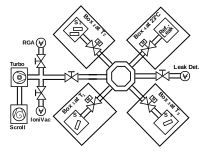
\includegraphics[width=.75\linewidth]{/Outgassing/Outgassing_experimental_setup_90_deg}
	\caption{.}
	\label{fig:outgassing_exp_setup}
\end{figure}

The remaining three vacuum chambers are used to investigate the out gassing rate of different glass samples. The stainless-steel chambers are conically shaped to minimize the contact between the glass-sample surfaces and the steel of the vacuum chamber. This allows the detection of Helium out gassing from all sample surfaces. The samples, together with the Helium-reference leak, are periodically exposed to the rest of the vacuum system and the quadruple mass spectrometer by opening and closing electric valves which are directly connected to the individual sample vacuum chambers. By cycling through the measurement chambers one can detect very small out gassing rates since the gas accumulates inside the sample chamber while the electric valves are closed. The pent-up gas is then released into the vacuum system and can be smoothly detected by the mass spectrometer once the respective electric valve is opened. The periodicity can be adjusted to the individual out gassing rates of the sample as well as the sample size, which both greatly influence the measurement signal detected by the Quadruple mass spectrometer. A greater accumulation time (or measurement period) would generally result in a much higher detected signal and the optimal accumulation time was adjusted before the measurement campaign by trial and error and turned out to be in the order of 200 seconds for the given Zerodur samples.\\\\
\noindent

\subsection{Sample preparation}
To load the Zerodur samples with Helium a secondary experimental setup is required (see Fig.\ref{fig:outgassing_exp_setup_for_loading}). To allow for a throughout permeation of Helium into the glass, the sample chamber is kept under a Helium atmosphere of 5 bars for six weeks before the actual measurement campaign begins. The loading time was chosen based on the out gassing time constant of Zerodur, which was on the order of two weeks. The time constant was experimentally determined in a preliminary experiment. Loading the the glass sample for more than three time constant ensures a fully loaded sample with a small Helium concentration gradient within the sample. \\ \\
\noindent
\begin{figure}[H]
	\centering
	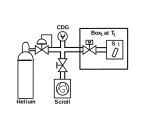
\includegraphics[width=.65\linewidth]{/Outgassing/Outgassing_experimental_setup_Sample_loading}
	\caption{.}
	\label{fig:outgassing_exp_setup_for_loading}
\end{figure}

\section{Experimental results}
Fig.\ref{fig:outgassing_cycle_example} shows the partial Helium pressure (in mbars) measured with the QMS for two consecutive measurement cycles, 50 days after the measurement campaign has begun. One can observe three distinct peaks which indicate the release of the pent-up Helium gas, from the individual sample chambers, into the evacuated vacuum system.
The Turbo pump removes the access gas from the system within 20 seconds and a plateau can be observed, which depends on the individual out gassing rate of the sample (or calibrated Helium Leak) and the pumping speed of the turbo pump which is continuously operating during the experiment. The partial pressure of each plateau is measured for roughly 60 seconds before the respective valve is closed and another sample chamber is opened. After opening the first sample chamber, which contains two identical Zerodur samples, an empty reference chamber is unlocked to determine the out gassing rate of an empty chamber for later offset correction of the measurement signal. The cycle continuous with the second measurement chamber opening, which contains one Zerodur sample. The valve is closed and the empty reference chamber is measured again before the cycle concludes with an observation of the reference chamber. Each individual measurement cycle takes 320 seconds to complete and is periodically repeated.\\\\
\noindent

\begin{figure}[H]
	\centering
	\includegraphics[width=.9\linewidth]{/Outgassing/RGA_Measurement_Cycle_Zerour_beschriftet}
	\caption{.}
	\label{fig:outgassing_cycle_example}
\end{figure}


To determine the out gassing rate of the samples, the measured plateaus were averaged over their respective measurement period and then plotted over time. Fig.\ref{fig:outgassing_Raw_data_outgassing_Zerodur} shows the result and the time dependent evolution of the QMS signal for the four connected sample or reference chambers. The second measurement chamber, which contains two identical Zerodur samples, was connected 38 (~ one time constant) days after the beginning of the overall measurement campaign. An initial multi-exponential decline of the RGA-signal is observed, while the signal of the chamber containing only one Zerodur-glass sample reached the characteristic mono-exponential He-out-gassing, which can generally be observed after more than one time constants has passed since the beginning of the experiment.\\\\
\noindent


\begin{figure}[H]
	\centering
	\includegraphics[width=.9\linewidth]{/Outgassing/RGA_Measurement_over_40days_Zerour}
	\caption{.}
	\label{fig:outgassing_Raw_data_outgassing_Zerodur}
\end{figure}

The respective He-out-gassing rate of the samples can be assessed from the RGA-signals after a normalization and offset correction was performed. The signal of the empty reference chamber was subtracted from the two sample-chamber QMS signals and afterwards normalized with the detected Helium reference leak signal for the respective measurement cycle. The offset-corrected and normalized signal can then be multiplied with the known He-out-gassing rate of the He-Leak to determine the overall He-out-gassing rates of the two respective sample chambers. \\\\
\noindent
\begin{figure}[H]
	\centering
	\includegraphics[width=.9\linewidth]{/Outgassing/RGA_Measurement_over_40days_Zerour_corrected_with_HE_Leak}
	\caption{.}
	\label{fig:outgassing_result_one_and_two_Zerodur_samples}
\end{figure}

The exponentially decaying data set can be fitted to determine the time constant $t_{out}$ and together with eq.(\ref{outgassing_timeconstant}) one can calculate the diffusion constant $D$ of Zerodur at 23$^\circ$C. Using eq.(\ref{outgassing_rate}) in combination with the results for $D$ one can calculate the initial Helium concentration $c_0$ of the sample and the Solubility $S$ of the material. Table(\ref{table:results_outgassing}) shows the combined results for the Zerodur samples investigated within the first measurement campaign.

\begin{table}[H]
	\begin{center}
		\begin{tabular}{ lllll }
			\toprule
			Sample name : & $t_{out}$ in days  &$Q_{out,(t=0)}$ in Pa m$^3$/s & $c_0$ Pa m$^3$/m$^3$ & S in ppm \\
			\midrule
			One Zerodur plate: &$35.57$& $1.31 \cdot 10^{-5}$& $7.144$ &  $14.28$\\
			Two Zerodur plates: &X&X&X&X\\
			\bottomrule
		\end{tabular}
	\end{center}
	\caption{.}
	\label{table:results_outgassing}
\end{table}
